\documentclass[11pt, A4paper, openany, uplatex]{book}
\usepackage[dvipdfmx, colorlinks = true, linkcolor = blue, filecolor = blue, urlcolor = blue, citecolor = blue]{hyperref}
\usepackage[dvipdfmx]{graphicx}
\usepackage[dvipdfmx]{color}
\usepackage{amsfonts}
\usepackage{amssymb}
\usepackage{amsmath}
\usepackage{ascmac}
\usepackage{framed}
\usepackage{comment}
\usepackage{latexsym}
\usepackage{endnotes}
\usepackage{mathrsfs}
\usepackage{longtable}
\usepackage[left=2.2cm,top=2cm,right=2.2cm,bottom=2cm]{geometry}
\usepackage{theorem}
\usepackage{lscape}
\usepackage{bm}
\usepackage{url}
\usepackage{listings}
\usepackage{makeidx}
\usepackage[titletoc]{appendix}
\usepackage{fdsymbol}

\DeclareMathOperator*{\plim}{plim}

\newcommand{\mbf}{\mathbf}
\newcommand{\mcl}{\mathcal}
\newcommand{\mbb}{\mathbb}
\newcommand{\mrm}{\mathrm}
\newcommand{\msc}{\mathscr}
\newcommand{\tr}{\top}
\newcommand{\eps}{\varepsilon}
\newcommand{\what}{\widehat}
\newcommand{\wtil}{\widetilde}
\newcommand{\R}{\textbf{R}}
\newcommand{\E}{\mathbb{E}}
\newcommand{\Var}{\mathrm{Var}}
\newcommand{\Cov}{\mathrm{Cov}}

\renewcommand{\hat}{\widehat}
\renewcommand{\tilde}{\widetilde}
\renewcommand{\bar}{\overline}


\newtheorem{theorem}{Theorem}[section]
\newtheorem{acknowledgement}[theorem]{Acknowledgement}
\newtheorem{algorithm}[theorem]{Algorithm}
\newtheorem{axiom}[theorem]{Axiom}
\newtheorem{case}[theorem]{Case}
\newtheorem{claim}[theorem]{Claim}
\newtheorem{conclusion}[theorem]{Conclusion}
\newtheorem{condition}[theorem]{Condition}
\newtheorem{conjecture}[theorem]{Conjecture}
\newtheorem{corollary}[theorem]{Corollary}
\newtheorem{criterion}[theorem]{Criterion}
\newtheorem{definition}[theorem]{Definition}
\newtheorem{example}[theorem]{Example}
\newtheorem{exercise}[theorem]{Exercise}
\newtheorem{lemma}[theorem]{Lemma}
\newtheorem{notation}[theorem]{Notation}
\newtheorem{problem}[theorem]{Problem}
\newtheorem{proposition}[theorem]{Proposition}
{\theorembodyfont{\upshape}
\newtheorem{remark}{Remark}
}
\newtheorem{solution}[theorem]{Solution}
\newtheorem{summary}[theorem]{Summary}
\newenvironment{proof}[1][Proof]{\textbf{#1.} }{\  \rule{0.5em}{0.5em}}
\newtheorem{assumption}{Assumption}
\oddsidemargin=0cm \evensidemargin=0cm
\numberwithin{equation}{section}
\def \baselinestretch{1.4}

\newcommand{\indep}{\mathrel{\text{\scalebox{1.07}{$\perp\mkern-10mu\perp$}}}}
\DeclareMathOperator*{\argmin}{\arg\!\min}
\DeclareMathOperator*{\argmax}{\arg\!\max}
\DeclareMathOperator*{\argsup}{\arg\!\sup}
\DeclareMathOperator*{\arginf}{\arg\!\inf}

\allowdisplaybreaks
\begin{document}
%%%%%%%%%%%%%%%%%%%%%%%%%%%%%%%%%%%%%%%%
\part{Econometric Analysis of Cross-Sectional Dependence Models}
%%%%%%%%%%%%%%%%%%%%%%%%%%%%%%%%%%%%%%%%
\chapter{Cross-Sectional Dependence}
\begin{center}
	\textit{Humans are social animals} (Aristotle).
\end{center}
\section{Social interaction}
We cannot live alone away from other people.
Our behavior is inevitably affected by those around us and the social groups we belong to, and vice versa.
This interaction with others is called \textbf{social interaction\index{social interaction}}.
Thus, in order to precisely understand the nature of human behavior, such feature, i.e. social interaction, should not (or often cannot) be overlooked.

In the literature of econometrics, there is a long history in modeling the dependence structure of time series data -- the interactions between the past and present.
Estimation of econometric models with social interactions (i.e., ``cross-sectional'' interactions) is a relatively young research theme (as compared to time series literature), and now growing attention has been devoted to this field.

In an early seminal paper, \cite{manski1993identification} considered a linear social interaction model, which is called a \textbf{linear-in-means model\index{linear-in-means model}}, and distinguished three types of effects among the social interaction effects: an individual's outcome can be affected by the average outcome in the group to which he/she belongs (\textbf{endogenous effects\index{endogenous effects}}), by the average individual characteristics in the group (\textbf{contextual effects\index{contextual effect}}), and by the common environment of the group (\textbf{correlated effects\index{correlated effects}}).

For example, consider a student's academic achievement as the dependent variable of interest, say, $Y$.
Let $X$ be a determinant of academic achievement, such as whether or not belonging to an academic club.
Further, denote $e$ as the quality of class teacher.
There is an endogenous effect if individual achievement $Y$ tends to vary with the mean achievement $\bar{Y}$ of the students in the same school, class room, or other reference groups ($\bar{Y} \to Y$).
Similarly, there is a contextual effect if achievement $Y$ tends to vary with $\bar{X}$, where $\bar{X}$ is, for example, the ratio of students belonging to academic clubs ($\bar{X} \to Y$).
There are correlated effects if the students in the same class tend to achieve similarly because they are taught by the same teacher ($e \to Y$).

Importantly, the three hypotheses have different policy implications.
Consider, for example, an educational intervention providing a tutoring program to some of the students but not to the others.
If the endogenous effect exists, then an effective tutoring program not only directly helps the tutored students but, as their achievement rises, indirectly helps  other students with a feedback to further achievement gains by the tutored students.
This is the so-called \textbf{spillover effect\index{spillover effect}} or \textbf{social multiplier effect\index{social multiplier effect}}.
Exogenous effects and correlated effects do not possess such multiplier mechanism.
Thus, identification of the three social interaction effects separately is of great importance to policy implementation and evaluation.
However, as described in Chapter \ref{chap:reflection}, this is not an easy task because of the so-called \textbf{reflection problem\index{reflection problem}}.

\section{Social network}

\textbf{Social network\index{social network}} is a type of platform that facilitates social interactions between individuals.
Here, the term ``social network'' is used to refer not only to the onilne SNS (social networking service), such as Facebook or Twitter, but to the connection of individuals in a broader sense (friendship, classmates, colleagues, international trade alliance, author-coauthor relationship, etc).
Mathematically, a social network can be represented by a directed or undirected \textbf{graph}, where individuals are represented as nodes/vertices and connections between them are represented as edges of the graph.
For example, Figure \ref{fig:GATT} shows the international trade network in 1954 (\cite{arpino2017implementing}).
The black edges indicate that both countries that are connected by the edge are members of the GATT (The General Agreement on Tariffs and Trade); gray edges indicate that at least one of the two countries is not a GATT member. 

\begin{figure}[h!]
	\begin{center}
		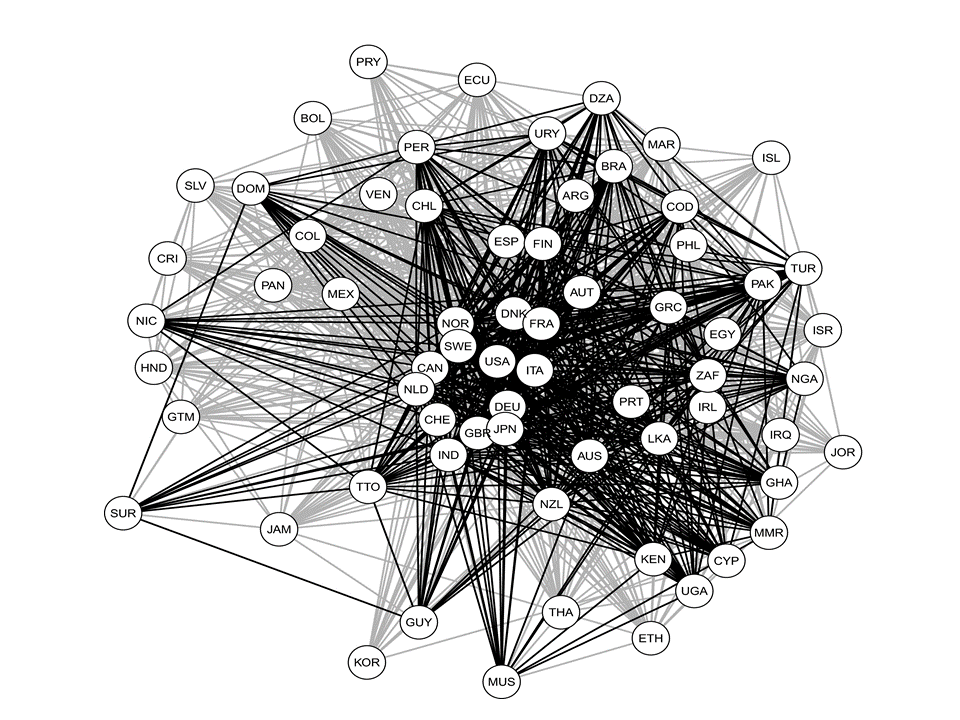
\includegraphics[width = 12cm]{GATT.png}
		\caption{Trade partners in 1954 and GATT membership, \cite{arpino2017implementing}.}
		\label{fig:GATT}
	\end{center}
\end{figure}

For another example, Figure \ref{fig:coauthor} shows the co-authorship network for 1,767 published papers in the field of statistics (\cite{said2010author}).

\begin{figure}[h!]
	\begin{center}
		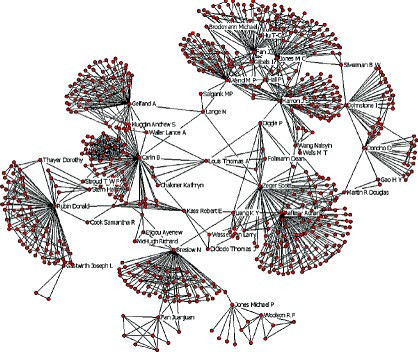
\includegraphics[width = 13cm]{coauthor.jpg}
		\caption{Co-authorship social network of statisticians, \cite{said2010author}.}
		\label{fig:coauthor}
	\end{center}
\end{figure}

Identification of linear-in-means social interaction models with network structure has been investigated by \cite{bramoulle2009identification}.
They show that, when social interactions are structured through a social network, endogenous and contextual effects can be identified (i.e., the reflection problem does not occur) on ``most'' networks.
This result will be described in detail in Chapter \ref{chap:social_network}.

\section{Spatial dependence}

Data of observations where each observation is identified by its geographical location is called spatial data. \textbf{Spatial dependence\index{spatial dependence}} (or, almost synonymously, \textbf{spatial autocorrelation\index{spatial autocorrelation}}) -- the tendency for nearby observations to be more highly correlated than those that are further apart -- distinguishes the analysis of spatial data from that of non-spatial data.
Spatial dependence is a common phenomenon observed in data from diverse areas such as climatology, geology, epidemiology, real estate market, crime, spatial price competition, etc. 

Figure \ref{fig:Tuberculosis} shows the spatial distribution of tuberculosis cases from 2002 to 2009 for each municipality in Brazil (\cite{harling2014spatial}).
In this figure, the higher rates of tuberculosis are found in the northwestern municipalities and in the coastal municipalities, indicating the presence of spatial dependence.

\begin{figure}[h!]
	\begin{center}
		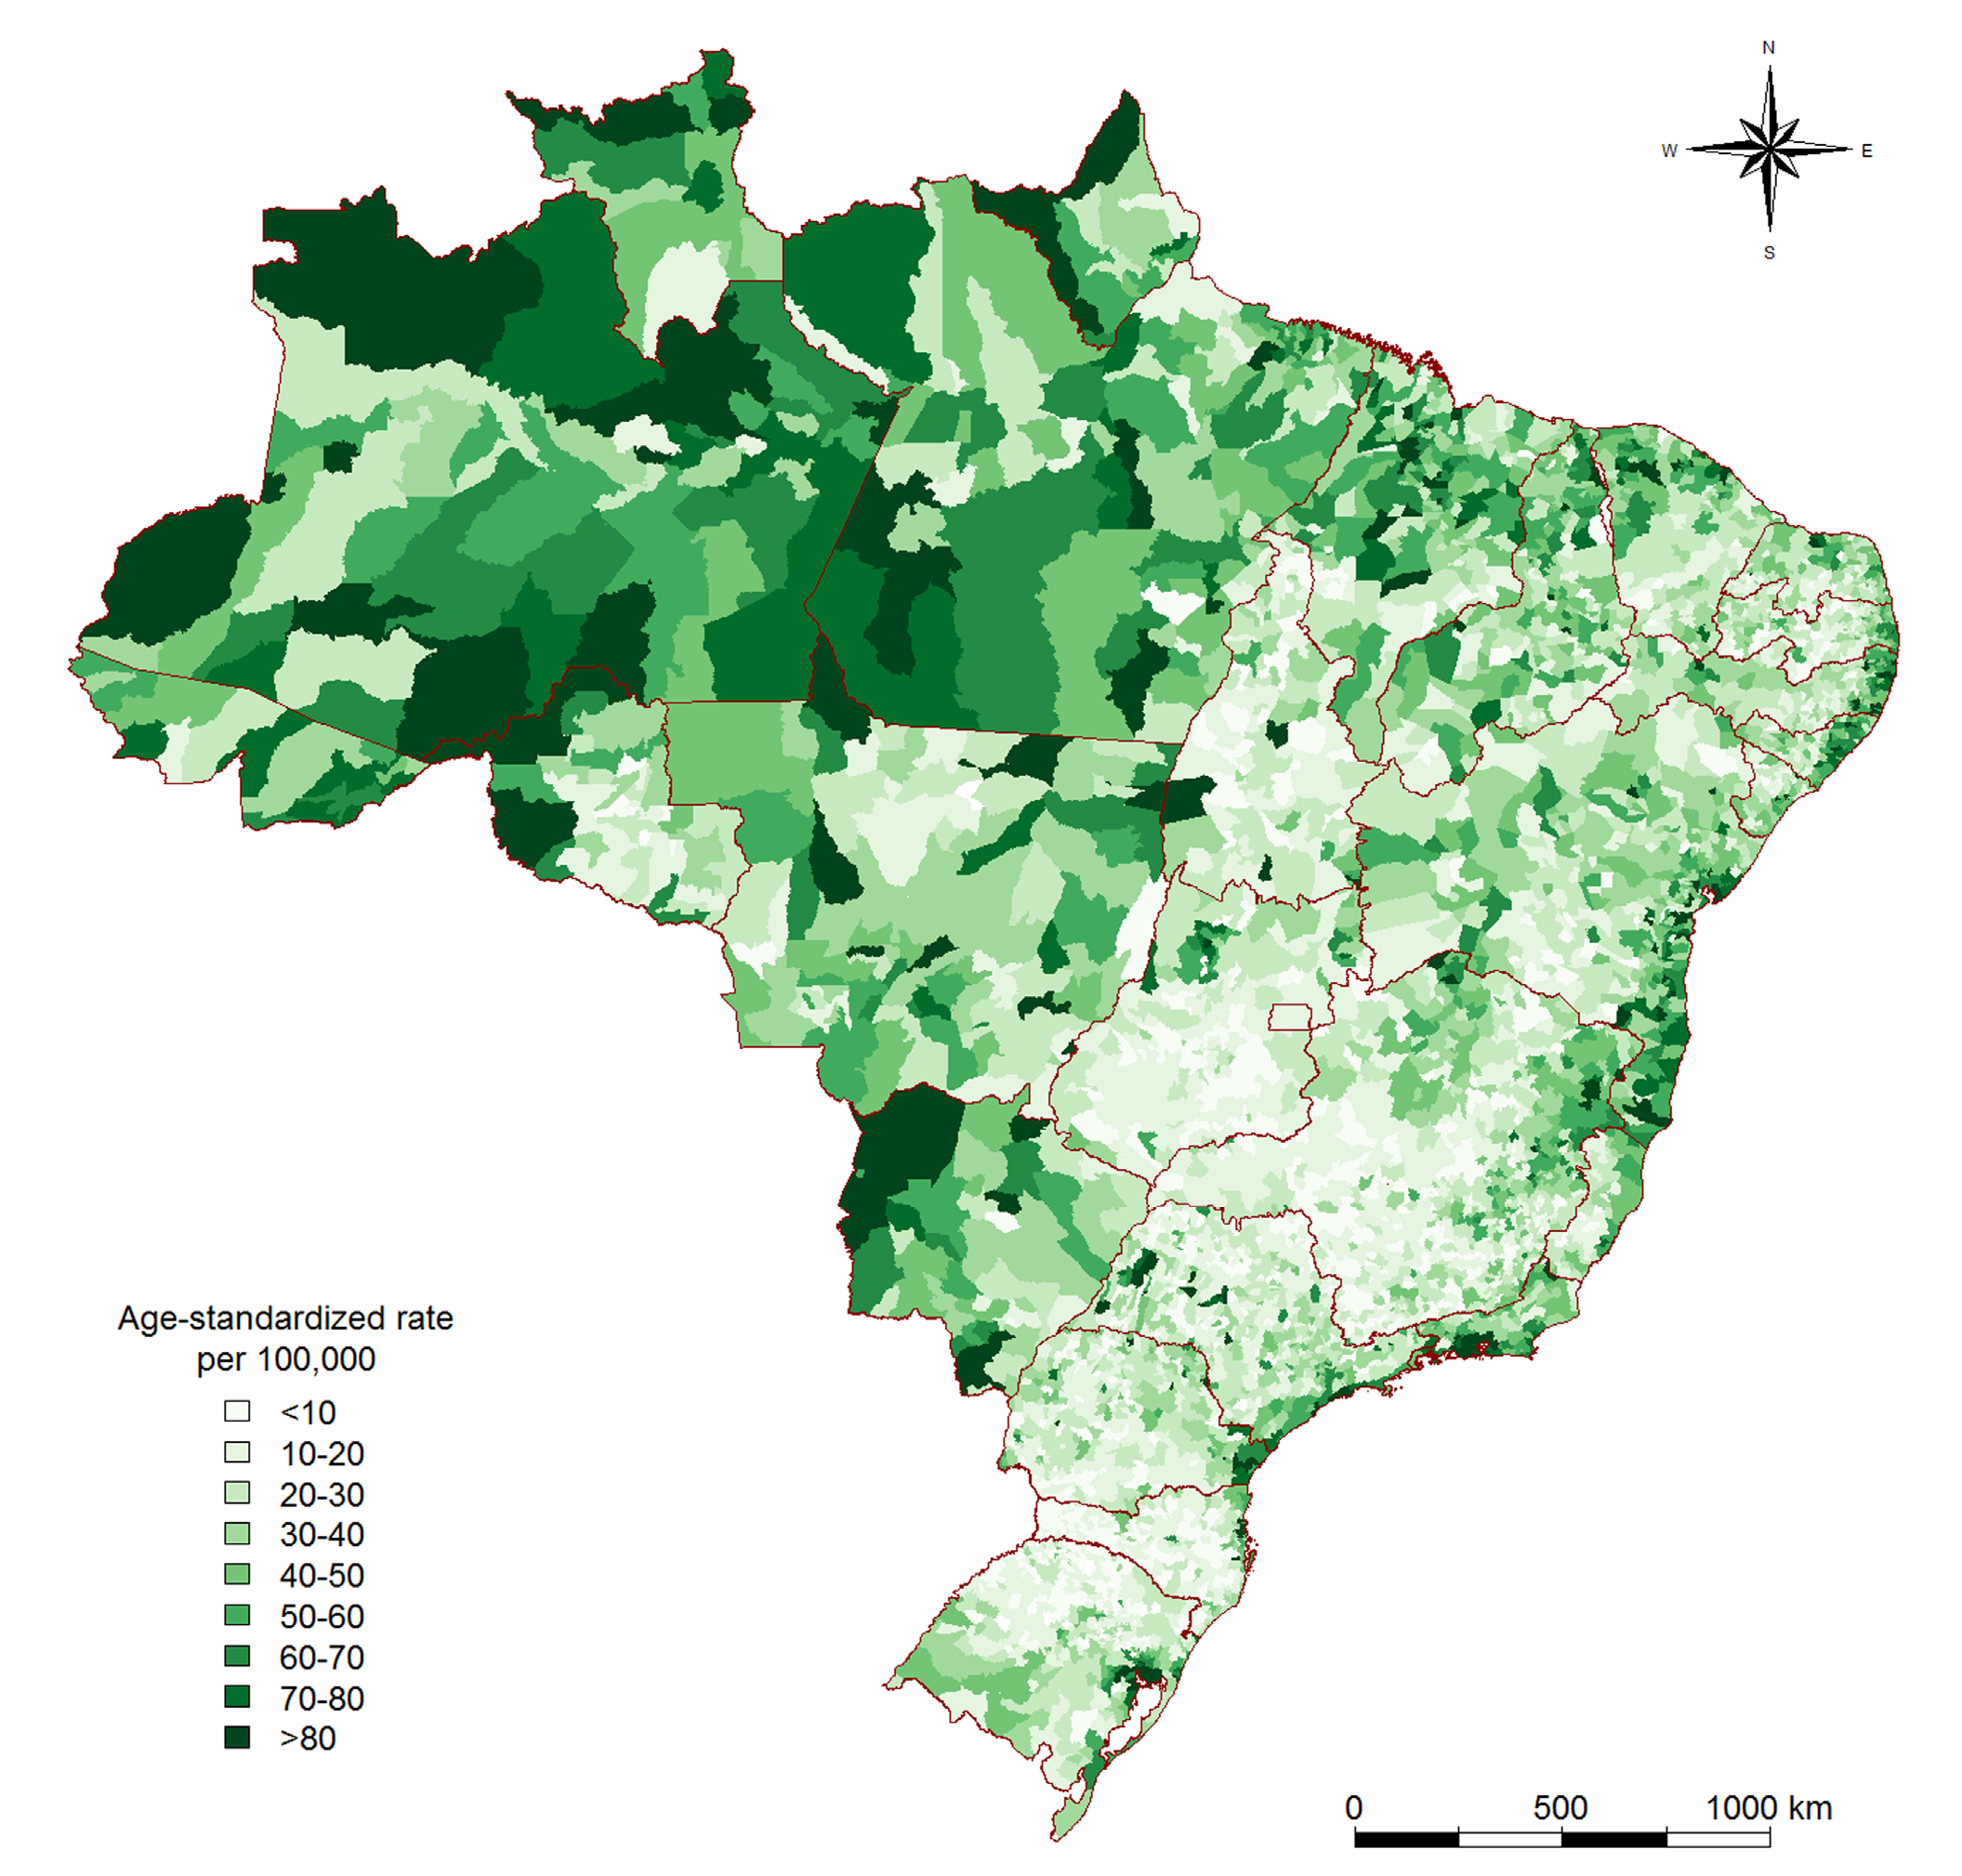
\includegraphics[width = 11cm]{Brazil.png}
		\caption{Municipal tuberculosis notification rates per 100,000 in Brazil 2002-2009, \cite{harling2014spatial}.}
		\label{fig:Tuberculosis}
	\end{center}
\end{figure}

\begin{figure}[h!]
	\begin{center}
		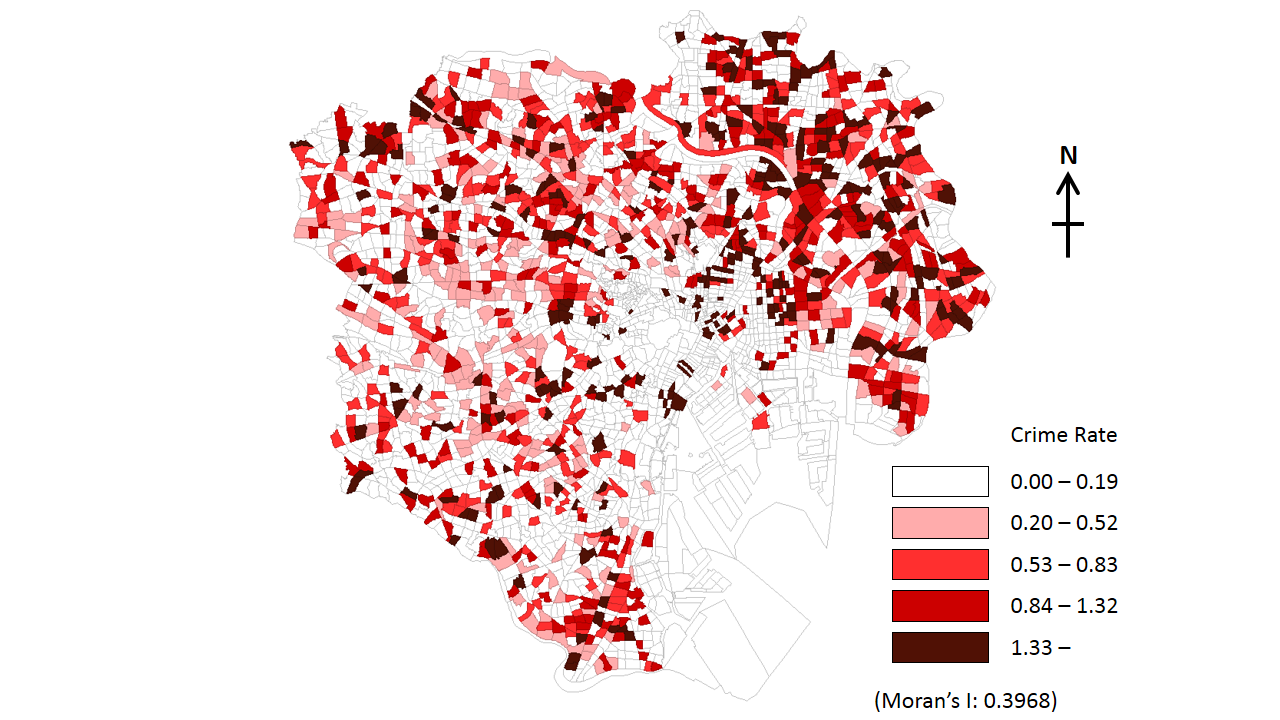
\includegraphics[width = 13cm]{crime.png}
		\caption{Distribution of household burglary rates in Tokyo 23-wards area 2011, \cite{hoshino2018semiparametric}.}
		\label{fig:crime}
	\end{center}
\end{figure}

Figure \ref{fig:crime} presents a map of Tokyo 23 wards and the value of the rate of household burglary per 1,000 households for each district in 2011 (\cite{hoshino2018semiparametric}).
The map indicates particularly low and high rates of household burglaries in the central and the northeast zones, respectively.
The \textbf{Moran's I} statistic, which is shown in the lower right of the figure (0.3968), is a type of correlation coefficient measuring the strength of spatial dependence, ranging from -1 (negative spatial dependence) to 1 (positive spatial dependence).
In Chapter \ref{chap:spatial_correlation}, we introduce several methods to statistically measure the degree of spatial correlation in data.

The field of statistics focusing on models that explicitly account for such spatial dependence is called \textbf{spatial statistics\index{spatial statistics}}, and particularly in the context of econometrics, it is called \textbf{spatial econometrics\index{spatial econometrics}}.
Since the pioneering work by \cite{anselin1988spatial}, spatial econometric methods have been widely applied in a number of empirical researches in economics.
An overview and introductory discussion of spatial econometric models are given in Chapters \ref{chap:spatial_econometrics} and \ref{chap:binary}.

One may have noticed that the spatial dependence can be seen as a special form of social interaction where the reference social group is formed based on geographical proximity.
Or, one can see social interaction as a special case of spatial dependence where the ``space'' is defined by social and economic distance between individuals.
Indeed, spatial econometric models and social interaction models have similarities in many aspects.

%%%%%%%%%%%%%%%%%%%%%%%%%%%%%%%%%%%%%%%%%%%%%%%%%%%%
%%%%%%%%%%%%%%%%%%%%%%%%%%%%%%%%%%%%%%%%%%%%%%%%%%%%
%%%%%%%%%%%%%%%%%%%%%%%%%%%%%%%%%%%%%%%%%%%%%%%%%%%%

\chapter{The Reflection Problem}\label{chap:reflection}
\section{Linear-in-means model}
\cite{manski1993identification} considered three hypotheses in order to explain the observation that individuals belonging to the same social group tend to behave similarly:
\begin{description}
	\item[Endogenous effects\index{endogenous effects}]  individuals' outcome can be affected by the mean outcome in the group.
	\item[Contextual effects\index{contextual effect}] individuals' outcome can be affected by the exogenous characteristics of the group (also referred to as \textbf{exogenous effects}).
	\item[Correlated effects\index{correlated effects}] individuals in the same group tend to behave similarly because they face similar institutional environments.
\end{description}

Let $Y$ be an outcome variable of interest (e.g., student's academic achievement), and $Z$ be a $K \times 1$ vector of individual characteristics. Also, let $X$ denote a $J \times 1$ vector of attributes characterizing an individual's reference group. Then, to account for the three distinct social effects, \cite{manski1993identification} considered the following model:
\begin{equation}\label{eq:lim1}
	Y = \alpha + \beta \E[Y \mid X] + \E[Z \mid X]^\top \gamma + Z^\top \eta + U, \quad \E[U \mid X, Z] = X^\top \delta 
\end{equation}
where $(\alpha, \beta, \gamma, \eta, \delta)$ are unknown parameters. The model in (\ref{eq:lim1}) is called the \textbf{linear-in-means model\index{linear-in-means model}}. It follows that the conditional expectation of $Y$ given $(X, Z)$ has the linear form
\begin{equation}\label{eq:lim2}
	\E[ Y \mid X, Z] = \alpha + \underbrace{\beta \E[Y \mid X]}_{\text{endogenous effect}} + \underbrace{\E[Z \mid X]^\top \gamma}_{\text{contextual effect}} + Z^\top \eta + \underbrace{X^\top \delta}_{\text{correlated effect}}
\end{equation}
If $\beta \neq 0$, $Y$ varies with $\E[Y \mid X]$, the mean of $Y$ among those individuals in the reference group characterized by $X$ (endogenous effect); if $\gamma \neq 0$, $Y$ varies with $\E[Z \mid X]$, the mean of $Z$ among those individuals in the reference group (contextual effect); and if $\delta \neq 0$, individuals in the reference group $X$ tend to behave similarly (correlated effect).

An important special case is when $X$ is a vector of indicator variables identifying which social group individuals belong to (i.e., $J$ groups in total). In this case, $\E[Y \mid X]$ and $\E[Z \mid X]$ simply denote the group means of $Y$ and $Z$, respectively, and $\delta$ represents the group-specific fixed effects.

\section{The reflection problem}

Taking the expectation of (\ref{eq:lim2}) with respect to $Z$ conditional on $X$ gives that $\E[Y \mid X]$ solves the  equation
\begin{equation}\label{eq:lim3}
	\E[Y \mid X] = \alpha + \beta \E[Y \mid X] + \E[Z \mid X]^\top (\gamma + \eta) + X^\top \delta 
\end{equation}
that is, $\E[Y \mid X]$ can be characterized as a fixed point of
\[
	H(p) \equiv \alpha + \beta p + \E[Z \mid X]^\top (\gamma + \eta) + X^\top \delta .
\]
If $\beta \neq 1$, we can solve (\ref{eq:lim3}) with respect to $\E[Y \mid X]$ as
\begin{equation}\label{eq:lim4}
	\E[Y \mid X] = \frac{\alpha}{1 -\beta} + \E[Z \mid X]^\top \frac{ (\gamma + \eta)}{1 - \beta} + X^\top \frac{\delta}{1 - \beta}. 
\end{equation}
Thus, $\E[Y \mid X]$ is a linear function of $(1, \E[Z \mid X], X)$, which implies that the endogenous effects can be expressed as the linear combination of the contextual effects and the correlated effects. Hence, in the linear-in-means model (\ref{eq:lim1}), the endogenous effects cannot be distinguished from the other two effects.

Specifically, inserting the right-hand side of (\ref{eq:lim4}) into (\ref{eq:lim2}) yields
\begin{align*}
	\E[Y \mid Z, X] 
	&= \alpha + \frac{\alpha \beta}{1 -\beta} + \E[Z \mid  X]^\top \left( \gamma +  \frac{\beta (\gamma + \eta)}{1 - \beta}\right) + Z^\top \eta  + X^\top \left( \delta + \frac{\delta \beta}{1 - \beta}\right)\\
	&= \frac{\alpha}{1 -\beta} + \E[Z \mid  X]^\top\frac{\gamma + \beta \eta}{1 - \beta} + Z^\top \eta + X^\top\frac{\delta}{1 - \beta}.
\end{align*}

\begin{theorem}[\cite{manski1993identification}]\label{thm:reflection}
Suppose that $\beta \neq 1$ and $(1, \E[Z \mid X], Z, X)$ are linearly independent.
Then, the composite parameters $(\alpha/(1 -\beta), (\gamma + \beta \eta)/(1 - \beta), \eta, \delta/(1 - \beta))$ are identified.
\end{theorem}

The interpretation of the theorem is as follows.
Suppose that a dataset $\{(Y_i, Z_i, X_i): 1 \le i \le n\}$ is available.
The theorem states that what we can estimate from the data are the four composite parameters: $\alpha/(1 -\beta)$, $(\gamma + \beta \eta)/(1 - \beta)$, $\eta$, and $\delta/(1 - \beta)$, no matter how large $n$ is.
On the other hand, the number of unknown parameters $(\alpha, \beta, \gamma, \eta, \delta)$ is five.
Therefore, we cannot identify these parameters uniquely (except for $\eta$).
In particular, the three social effects $(\beta, \gamma, \delta)$ cannot be distinguished.
This is called the \textbf{reflection problem\index{reflection problem}}.\footnote{
	Even in the presence of the reflection problem, if the value of $(\gamma + \beta \eta)/(1 - \beta)$ is non-zero, then either $\gamma$ or $\beta\eta$ (or both) is non-zero.
	Hence, one can still determine whether ``some'' social effects exist or not.
	}

If one has additional information on some parameter values, the identification result can be improved.
For example, suppose that contextual effects and correlated effects do not exist: $\gamma = \delta = 0$. Then, in this case, we have
\begin{align*}
	\E[Y \mid Z, X] = \frac{\alpha}{1 -\beta} + \E[Z \mid X]^\top\frac{\beta \eta}{1 - \beta} + Z^\top \eta .
\end{align*}
\begin{proposition}[\cite{manski1993identification}]\label{prop:reflection2} 
	Suppose that $\beta \neq 1$, $\gamma = \delta = 0$, and $(1, \E[Z \mid X], Z)$ are linearly independent. 
	Then, the composite parameters $(\alpha/(1 -\beta),  \beta \eta/(1 - \beta), \eta)$ are identified.
\end{proposition}

The proposition implies that, since $\eta$ is identified, the endogenous effect $\beta$ can be also identified from $\beta \eta / (1 - \beta)$ if $\eta \neq 0$.

\section{Numerical simulation with \R}

A direct consequence obtained from Theorem \ref{thm:reflection} and Proposition \ref{prop:reflection2} is that when $\gamma \neq 0$ the parameters of interest in model \eqref{eq:lim1}, except for $\eta$, cannot be estimated because $(1, \E[Y \mid X], \E[Z \mid X], Z)$ is linearly dependent; however, if both $\gamma$ and $\delta$ are zero, the parameters can be estimated.

We can check this result with a numerical simulation in \R.
The data-generating process used in the simulation is as follows.
\begin{lstlisting}[basicstyle=\ttfamily\footnotesize, frame=single]
N <- 300                             # sample size
X <- c(t(matrix(rnorm(10), 10, 30))) # 10 groups, 30 individuals for each.
Z <- X + X^2 + rnorm(N)              # E[Z | X] = X + X^2
U <- rnorm(N)                        # no correlated effect
 
alpha <- 1
beta  <- 0.5
gamma <- 1
eta   <- 1
 
EZ_X <- X + X^2
EY_X <- (alpha + EZ_X*(gamma + eta)) / (1 - beta)
Y    <- alpha + beta*EY_X + gamma*EZ_X + eta*Z + U
 \end{lstlisting}
The data are comprised of ten social groups with 30 members for each group, and thus, the total sample size is 300.
Here, we assume that there is no correlated effect, but the contextual effect is non-zero ($\gamma = 1$).
The conditional expectation of $Z$ given $X$ is given by $\E[Z \mid X] = X + X^2$, and that of $Y$ can be computed following equation \eqref{eq:lim4}.
Now, with this simulated dataset, if we run a linear regression of $Y$ on $(1, \E[Y \mid X], \E[Z \mid X], Z)$, ...
\begin{lstlisting}[basicstyle=\ttfamily\footnotesize, frame=single]
>  lm(Y ~ EY_X + EZ_X + Z)

Call:
lm(formula = Y ~ EY_X + EZ_X + Z)

Coefficients:
(Intercept)         EY_X         EZ_X            Z  
	 0.5158       0.7568           NA       1.0693 
\end{lstlisting}
we cannot obtain the estimate of $\gamma$ (\texttt{NA} stands for ``not available'').
If we reverse the order of $\E[Y \mid X]$ and $\E[Z \mid X], Z)$,
\begin{lstlisting}[basicstyle=\ttfamily\footnotesize, frame=single]
>  lm(Y ~ EZ_X + EY_X + Z)

Call:
lm(formula = Y ~ EZ_X + EY_X + Z)
	
Coefficients:
(Intercept)         EZ_X         EY_X            Z  
	  2.029        3.027           NA        1.069
\end{lstlisting}
now the value of $\beta$ becomes \texttt{NA}, implying that the social effects $\beta$ and $\gamma$ cannot be separately identified, i.e., the reflection problem.
However, note that the estimate of $\eta$ is unaffected by the order of regressors and is very close to its true value, that is, $\eta$ can be identified even  in the presence of the reflection problem.
This result is consistent with Theorem \ref{thm:reflection}.

Next, using the same dataset, we restrict the value of $\gamma$ to zero, as required in Proposition \ref{prop:reflection2}.
\begin{lstlisting}[basicstyle=\ttfamily\footnotesize, frame=single]
>  EY_X <- (alpha + EZ_X*eta) / (1 - beta)
>  Y    <- alpha + beta*EY_X + eta*Z + U
>  lm(Y ~ EY_X + Z)

Call:
lm(formula = Y ~ EY_X + Z)
	
Coefficients:
(Intercept)         EY_X            Z  
	 1.0022       0.5137       1.0693  
\end{lstlisting}
Then, we can estimate all parameters in the model correctly.

\section{A game theoretic interpretation}

We can interpret the linear-in-means model as a game theoretic model of incomplete information.
For simplicity, in this section we assume that contextual effects and correlated effects do not exist: $\gamma = \delta = 0$.

Let $q\in \mathbb{R}$ be an action, and the actual action made by individual $i$ is denoted by $Y_i$.
Now, assume that the payoff of individual $i$ choosing $q $ can be written as the following quadratic function:
\begin{equation*}
u_i(q, \{Y_j : X_j = X_i \})=\left[ \alpha + Z_i^\top \eta  + U_i \right] q -\frac{q^{2}}{2} + T_i(q, \{Y_j: X_j = X_i \}),
\end{equation*}
where $T_i(q, \{Y_j: X_j = X_i \})$ is a term representing the endogenous interaction between $i$ and the other members of the group to which $i$ belongs.  
For example, consider 
\begin{equation*}
T_i(q, \{Y_j : X_j = X_i \}) \equiv \dfrac{\beta}{|\{j : X_j = X_i \}|}\sum_{j : X_j = X_i}  Y_j q, \quad \beta > 0,
\end{equation*}
where $|A|$ denotes the cardinality of the set $A$.
This specification presumes that the source of social interactions is ``complementarity'': the average of group members' outcomes positively affects the individual's own marginal payoff.

Suppose that individual characteristics and error term, $Z_i$ and $U_i$, are unobservable to the other individuals including those in the same group. 
This implicitly postulates that each social group is sufficiently large such that the members of the group are not identifiable with each other.
Then, it is impossible to predict precisely the actual actions $\{Y_j: X_j = X_i \}$ from the point of view of $i$. In this situation, it is conventional to assume that each individual's behavior is characterized by a Bayesian--Nash equilibrium.
That is, a rational individual would choose an action to maximize her expected payoff:
\begin{align*}
	Y_i 
	&=\argmax_q \E_i \left[ u_i(q, \{Y_j : X_j = X_i \}) \right] \\
	&=\argmax_q \left\{ \left[ \alpha + Z_i^\top \eta  + U_i \right] q -\frac{q^{2}}{2} + \dfrac{\beta}{|\{j : X_j = X_i \}|}\sum_{j : X_j = X_i}  \E_i[Y_j] q \right\} \\
	&= \alpha + \dfrac{\beta}{|\{j : X_j = X_i \}|}\sum_{j : X_j = X_i}  \E_i[Y_j] + Z_i^\top \eta  + U_i,
\end{align*}
where $\E_i[Y_j]$ is the conditional expectation of $Y_j$ given the information set of $i$.
Notice that, because we have assumed that $Z_j$ and $U_j$ are unknown to $i$, they are not included in $i$'s information set.
Further, if $(Z, U)$'s are independent among individuals, the only available information to compute $\E_i[Y_j]$ is that $j$ is in the same group as $i$.
Consequently, we may have $\E_i[Y_j] = \E[Y | X = X_i]$; this results in the linear-in-means model:
\[
	Y_i = \alpha + \beta \E[Y | X = X_i] + Z_i^\top \eta  + U_i.
\]

The linear-in-means model assumes that an individual is affected equally by all the other members of the same group, and that she forms beliefs about their behavior utilizing only the group-level covariates.
As suggested in \cite{lee2014binary}, such framework is not appropriate for, for example, friendship networks, where the size of each social group is relatively small.
When the size of group is small, the values of the individuals characteristics $Z$ of those in the same group would be common knowledge within the members; that is $\E_i[Y_j] = \E[Y \mid Z = Z_j, X = X_i]$.
\cite{lee2014binary} called this paradigm of belief formation ``heterogeneous rational expectations''.
Heterogeneous rational expectations imply that the predicted value of the outcome of different members with different individual characteristics will be different. 
For more details, see their paper.


%%%%%%%%%%%%%%%%%%%%%%%%%%%%%%%%%%%%%%%%%%%%%%%%%


\chapter{Social Interactions through Social Networks}\label{chap:social_network}
\section{Common types of social network graphs}

\textbf{Social network\index{social network}} is a type of platform that facilitates social interactions between individuals. 
In social network analysis, networks are typically represented as \textbf{graphs\index{graph}}.
The followings are examples of social networks that we often observe in real data.
\textit{Facebook}: an undirected graph (a mutual consent is required to become Friends), \textit{Twitter}: a directed graph (a mutual consent is not required to be a Follower), \textit{married couples}: a disconnected undirected graphs, \textit{leader and followers}: a directed star graph, \textit{classroom membership}: a complete graph, and so forth.

\begin{figure}[h!]
	\begin{center}
		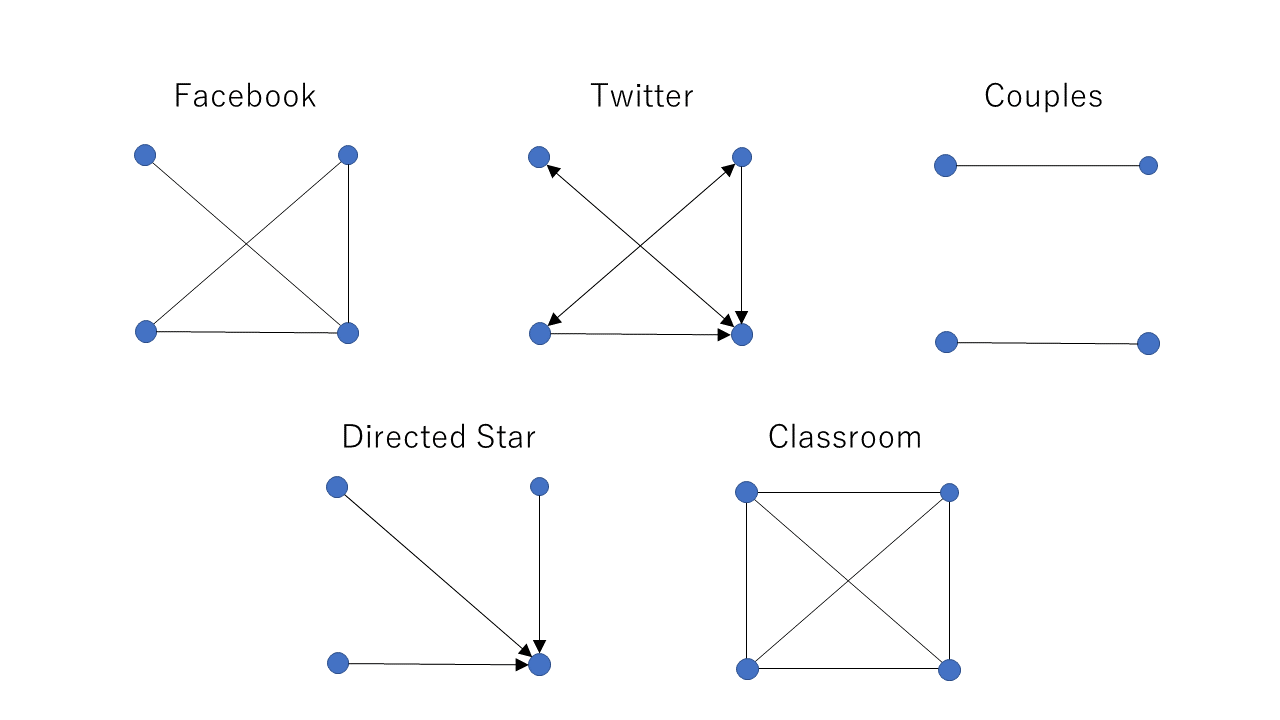
\includegraphics[width = 14cm]{snets.png}
		\caption{Social network graphs}
	\end{center}
\end{figure}

\section{Linear-in-means social network model}

When social interactions occur on social networks, such as friendship networks, the reference group for each individual is formed by the agents who are connected to her.
Thus, since the members of the reference group are distinguishable in this situation (unless the reference group is extremely large), Manski's linear-in-means model would not be appropriate.

Suppose there is a sample of $n$ individuals that form social networks.
Each individual $i$ belongs to one of these  groups, and $i$ does not necessarily interact with all the members of the group to which $i$ belongs, but may have a specific reference group (close friends) $P_i$ of size $n(i)$. 
Individual $i$ is excluded from her own reference group $P_i$, that is, $ i \not\in P_i$.
The reference is either directed  or undirected. 
For both cases, if $j$ affects $i$, we obtain $j \in P_i$.
When the friendship is directed, $j \in P_i$ does not imply the converse $i \in P_j $.
We say that an individual $i$ is \textbf{isolated\index{isolated}} if $P_i$ is empty. 
Note that while an isolated individual is not affected by the other individuals, she can still affect the others if the reference is asymmetric.
Throughout this section, we assume that not all individuals are isolated. 

\begin{figure}[h!]
	\begin{center}
	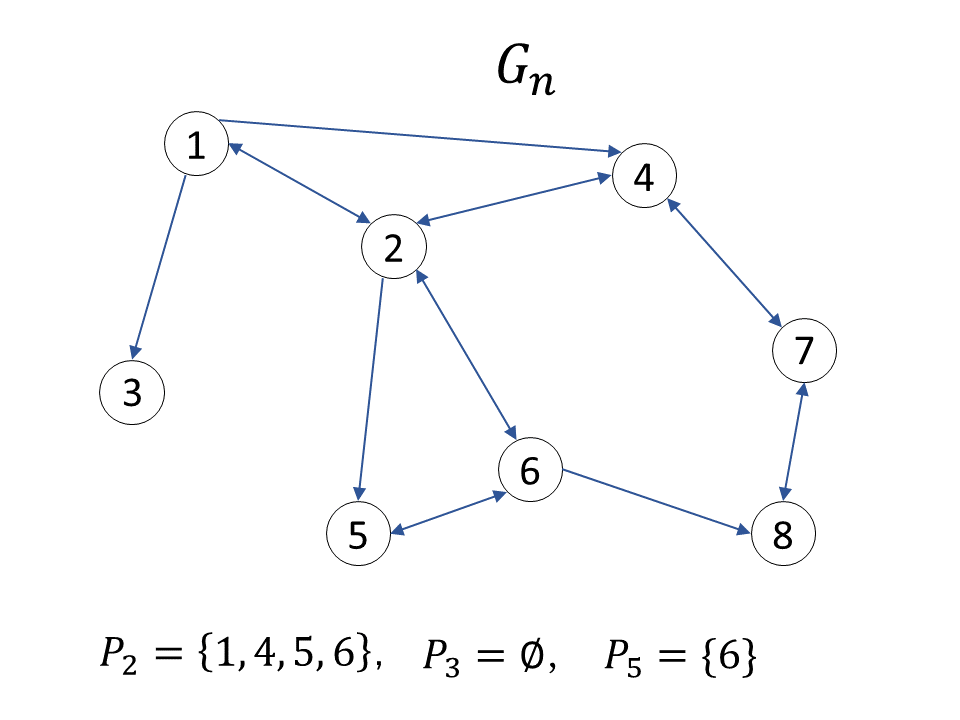
\includegraphics[width = 8cm]{reference.png}
	\caption{Reference groups. The arrows represent friendship nominations.}
	\end{center}
\end{figure}

Let $Y$ be an outcome variable of interest, and $X$ be the vector of individual characteristics. Then, we consider the following linear-in-means social network model (\cite{bramoulle2009identification}):
\begin{align}\label{eq:bramoulle}
	Y_i = \alpha + \beta \frac{\sum_{j \in P_i} Y_j}{n(i)} + X_i^\top \gamma +  \frac{\sum_{j \in P_i} X_j^\top}{n(i)} \delta + \epsilon_i, 
\end{align}
where $\beta$ captures the endogenous effect and $\delta$ the contextual effect.
For simplicity of discussion, we do not consider the correlated effects here.\footnote{
	In the linear-in-means social network models as in \eqref{eq:bramoulle}, one can account for the correlated effects by including  \textit{network fixed effects} in the model.
	For more details, see, for example, \cite{lee2007identification} and \cite{bramoulle2009identification}.
	}
The conditional expectation of $\epsilon$ given $\mathbf{X}_n = (X_1, \ldots, X_n)^\top$ is assumed to be zero: $\E[\epsilon \mid \mathbf{X}_n] = 0$ (i.e., $X$ is exogenous).

Let $\underset{n \times n}{G_n}$ be the weighted social interaction matrix (this is a directed adjacency matrix weighted by $n(i)^{-1}$).\footnote{
	Throughout this chapter, we assume that $G_n$ is non-stochastic.
	However, this assumption is indeed debatable.
	Identification and estimation of social interaction models with stochastic and endogenous $G_n$ is an important research topic in the recent literature.
}
Namely, the $(i,j)$-th element of $G_n$ is given by
\begin{align*}
	 (G_n)_{i,j} = \left\{\begin{array}{ll}
	1/n(i) & \text{ if } j \in P_i \\
	0 & \text{ otherwise }
	\end{array}\right.
\end{align*}
Note that the sum of each $i$'s row of $G_n$ is one, unless $i$ is isolated.
We can write model \eqref{eq:bramoulle} in matrix form as
\begin{align}\label{eq:bramat}
	\mbf{Y}_n = \alpha \mathbf{1}_n + \beta G_n \mbf{Y}_n + \mbf{X}_n \gamma +  G_n \mbf{X}_n \delta + \mcl{E}_n, 
\end{align}
where $\mbf{1}_n$ is an $n\times 1$ vector of ones, $\mbf{Y}_n = (Y_1, \ldots, Y_n)^\top$, and $\mcl{E}_n = (\epsilon_1, \ldots, \epsilon_n)^\top$.
Throughout the rest, we assume that $(\mathbf{1}_n, \mbf{X}_n)$ is linearly independent.

\paragraph{A game theoretic interpretation}

As opposed to Manski's linear-in-means model,  the model in \eqref{eq:bramoulle} can be seen as a game theoretic model of ``complete information''.
Assume that the payoff of individual $i$ choosing an action $q \in \mbb{R}$ can be written as the following quadratic function:
\begin{equation*}
u_i(q, \{Y_j\}_{j \in P_i})=\left[ \alpha + X_i^\top \gamma +  \frac{\sum_{j \in P_i} X_j^\top}{n(i)} \delta + \epsilon_i  \right] q -\frac{q^{2}}{2} + \beta \frac{\sum_{j \in P_i} Y_j}{n(i)} q, \;\; \beta > 0.
\end{equation*}
Here, $Y_j$'s, $j \in P_i$, are observable to $i$ under complete information. 
This specification presumes that the source of social interactions is \textbf{complementarity\index{complementarity}}: the average of friends' outcomes positively affects the individual's own marginal payoff.
Then, based on the payoff-maximization principle, the set of realized outcomes $\{Y_1, \ldots, Y_n\}$ can be characterized by a pure Nash equilibrium.
That is, 
\begin{align*}
	Y_i 
	&= \argmax_{q \in \mbb{R}}u_i(q, \{Y_j\}_{j \in P_i}) \\
	&= \alpha + \beta \frac{\sum_{j \in P_i} Y_j}{n(i)} + X_i^\top \gamma +  \frac{\sum_{j \in P_i} X_j^\top}{n(i)} \delta + \epsilon_i
\end{align*}
for all $i = 1, \ldots, n$.

For another example, one can consider
\begin{equation*}
u_i(q, \{Y_j\}_{j \in P_i})=\left[ \alpha + X_i^\top \gamma +  \frac{\sum_{j \in P_i} X_j^\top}{n(i)} \delta + \epsilon_i  \right] q -\frac{q^{2}}{2} -\frac{\beta}{2} \left( q - \dfrac{\sum_{j \in P_i} Y_j}{n(i)} \right)^2, \;\; \beta > 0.
\end{equation*}
In this case, the source of social interactions is described by \textbf{conformity\index{conformity}}: $i$'s payoff is positively affected by the degree to which she conforms with her close friends' actions. 
Solving the payoff-maximization problem, we can find that we obtain the same model as in \eqref{eq:bramoulle}.
This implies that it is generally impossible to identify the source of social interactions from model \eqref{eq:bramoulle}. 

\section{Using network structure to identify social interactions}

In the following, assume that $|\beta| < 1$.
Then, we can show that the inverse matrix $(I_n - \beta G_n)^{-1}$ exists.
For simplicity of presentation, assume that the dimension of $X$ is equal to one: $\mrm{dim}(X) = 1$.
Then, the ``reduced-form'' of model \eqref{eq:bramat} can be written as
\begin{align*}
	\mbf{Y}_n 
	& = \alpha (I_n - \beta G_n)^{-1}\mathbf{1}_n  + \gamma (I_n - \beta G_n)^{-1}\mbf{X}_n  + \delta (I_n - \beta G_n)^{-1} G_n \mbf{X}_n + (I_n - \beta G_n)^{-1}\mcl{E}_n\\
	& =  \alpha (I_n - \beta G_n)^{-1}\mathbf{1}_n  + (I_n - \beta G_n)^{-1}( \gamma I_n + \delta G_n ) \mbf{X}_n + (I_n - \beta G_n)^{-1}\mcl{E}_n.
\end{align*}
Note that it follows from the Neumann series expansion (Lemma \ref{lem:neumann}) that 
\begin{align*}
	 (I_n - \beta G_n)^{-1} 
	& = I_n + \beta G_n + \beta^2 G_n G_n + \beta^3 G_n G_n G_n + \cdots \\
	&= \sum_{t = 0}^\infty \beta^t G_n^t,
\end{align*}
where $G_n^0 = I_n$.
Thus, we have 
\[
	(I_n - \beta G_n)^{-1}\mbf{X}_n = \mbf{X}_n + \beta G_n \mbf{X}_n + \beta^2 G_n^2\mbf{X}_n + \cdots,
\]
where the first term on the right-hand side is the individual's own characteristic variables, the second term represents the average characteristics of her direct friends multiplied by $\beta$, the third term is the average characteristics of friends' friends multiplied by $\beta^2$, and so forth (see also Appendix \ref{sec:adjacency}).
This implies that, if $\beta \neq 0$, the characteristics of other individuals in the same network can affect own outcome through the social interactions, even when they are not her direct friends, and, conversely, her own characteristics affect the outcomes of the others in the same network.
In this sense, the matrix $(I_n - \beta G_n)^{-1} $ is often called the \textbf{social multiplier} matrix.

Here, assume that there are no isolated individuals.
In this case, all row-sums of $G_n^t$ for all $t = 0, 1, \ldots$ are equal to one.
Therefore, it holds that
\begin{align}\label{eq:intercept}
	\alpha  (I_n - \beta G_n)^{-1} \mathbf{1}_n 
	= \alpha \sum_{t = 0}^\infty \beta^t G_n^t \mathbf{1}_n 
	= \alpha  \sum_{t = 0}^\infty \beta^t \mathbf{1}_n  = \frac{\alpha}{1 - \beta}\mathbf{1}_n .
\end{align}
\bigskip

Now, let $\theta = (\alpha, \beta, \gamma, \delta)$ be the vector of unknown parameters to be estimated.
We say that the matrices $I_n$, $G_n$, and $G_n^2$ are linearly independent if and only if
\[
	\mu_0 I_n + \mu_1 G_n + \mu_2 G_n^2 = 0
\]
implies that $\mu_0 = \mu_1 = \mu_2 = 0$.
\begin{proposition}[\cite{bramoulle2009identification}]\label{prop:bra}
	Suppose that $\gamma \beta + \delta \neq 0$.
	
	(i)  If the matrices $I_n$, $G_n$, and $G_n^2$ are linearly independent, $\theta$  is identified.
	
	(ii) If the matrices $I_n$, $G_n$, and $G_n^2$ are linearly dependent and there are no isolated individuals, $\theta$ is not identified.
\end{proposition}

\begin{proof}
	(i) Consider two parameter vectors $\theta = (\alpha, \beta, \gamma, \delta)$ and $\theta' = (\alpha', \beta', \gamma', \delta')$.
	We show that
	\begin{align}\label{eq:ident1}
	\alpha (I_n - \beta G_n)^{-1}\mathbf{1}_n  + (I_n - \beta G_n)^{-1}( \gamma I_n + \delta G_n ) \mbf{X}_n = \alpha' (I_n - \beta' G_n)^{-1}\mathbf{1}_n  + (I_n - \beta' G_n)^{-1}( \gamma' I_n + \delta' G_n ) \mbf{X}_n
	\end{align}
	implies $\theta = \theta'$.
	Note that the above equality implies that 
	\begin{align*}
	& \alpha (I_n - \beta G_n)^{-1}\mathbf{1}_n = \alpha' (I_n - \beta' G_n)^{-1}\mathbf{1}_n\\
	& (I_n - \beta G_n)^{-1}( \gamma I_n + \delta G_n ) \mbf{X}_n = (I_n - \beta' G_n)^{-1}( \gamma' I_n + \delta' G_n ) \mbf{X}_n
	\end{align*}
	by the linear independence of $(\mbf{1}_n, \mbf{X}_n)$.
	Multiplying the both sides of the second equality by $I_n - \beta G_n$ yields
	\begin{align*}
	\gamma I_n + \delta G_n 
	& = (I_n - \beta G_n) (I_n - \beta' G_n)^{-1}( \gamma' I_n + \delta' G_n ) \\
	& = (I_n - \beta' G_n)^{-1}( \gamma' I_n + \delta' G_n )  - \beta G_n(I_n - \beta' G_n)^{-1}( \gamma' I_n + \delta' G_n ).
	\end{align*}
	Noting that $G_n(I_n - \beta' G_n)^{-1} = (I_n - \beta' G_n)^{-1} G_n$, further multiplying the both sides by $I_n - \beta' G_n$,
	\begin{align}
	& \gamma I_n + \delta G_n - \gamma \beta' G_n - \delta \beta' G_n^2 =  \gamma' I_n + \delta' G_n   - \gamma' \beta G_n   - \delta' \beta G_n^2 \nonumber \\
	& \Longrightarrow (\gamma - \gamma') I_n + (\delta - \delta' + \gamma'\beta - \gamma\beta' )G_n + (\delta'\beta - \delta\beta') G_n^2 =0. \label{eq:ident2}
	\end{align}
	Hence, we obtain $\gamma = \gamma'$, $\delta  + \gamma'\beta = \delta' + \gamma\beta'$ and $\delta'\beta = \delta\beta'$.
	Let $\lambda = \beta'/\beta$ such that $\beta' = \lambda \beta$ and $\delta' = \lambda \delta$.
	Then, 
	\begin{align*}
	\gamma = \gamma',\;\; \delta  + \gamma'\beta = \delta' + \gamma\beta' \quad 
	& \Longrightarrow\quad \delta  + \gamma \beta = \delta' + \gamma\beta' \\
	& \Longrightarrow \quad \delta  + \gamma \beta = \lambda (\delta + \gamma \beta) \\
	& \Longrightarrow \quad \lambda = 1 \quad (\because \gamma \beta + \delta \neq 0) \quad \Longrightarrow \quad \beta = \beta', \;\; \delta = \delta'.
	\end{align*}
	Finally, $\alpha = \alpha'$ follows from $\alpha (I_n - \beta G_n)^{-1}\mathbf{1}_n = \alpha' (I_n - \beta G_n)^{-1}\mathbf{1}_n$.
	
	(ii) When the matrices $I_n$, $G_n$, and $G_n^2$ are linearly dependent, we can find $\theta' = (\alpha', \beta', \gamma', \delta')$ that satisfy \eqref{eq:ident1} and \eqref{eq:ident2} but at least one of the following inequalities holds:
	\[
	\gamma - \gamma' \neq 0, \;\; \delta - \delta' + \gamma'\beta - \gamma\beta' \neq 0, \;\; \delta'\beta - \delta\beta' \neq 0.
	\]
	This implies that at least $\beta$ and $\delta$ cannot be separately identified.
	For the identification of $\alpha$, because no individual is isolated,
	\[
	\alpha (I_n - \beta G_n)^{-1}\mathbf{1}_n = \alpha' (I_n - \beta' G_n)^{-1}\mathbf{1}_n \iff \alpha/(1 - \beta) = \alpha'/(1 - \beta')
	\]
	by \eqref{eq:intercept}.
	Since $\beta$ is not identified, $\alpha$ is also not identified.
\end{proof}
\bigskip

In Proposition \ref{prop:bra}, we have assumed that $\gamma \beta + \delta \neq 0$.
The role of this assumption should be clear from the following equality.
Noting that $(I_n - \beta G_n)^{-1} = I_n +  \beta G_n(I_n - \beta G_n)^{-1}$, if $\gamma \beta + \delta = 0$, we have
\begin{align*}
	\E[\mbf{Y}_n \mid \mbf{X}_n] 
	& = \alpha (I_n - \beta G_n)^{-1}\mathbf{1}_n + \gamma (I_n - \beta G_n)^{-1}\mbf{X}_n + \delta (I_n - \beta G_n)^{-1}G_n \mbf{X}_n\\
	& = \alpha (I_n - \beta G_n)^{-1}\mathbf{1}_n + \mbf{X}_n \gamma +  (\gamma \beta + \delta) (I_n - \beta G_n)^{-1}G_n \mbf{X}_n \\
	& = \alpha (I_n - \beta G_n)^{-1}\mathbf{1}_n + \mbf{X}_n \gamma.
\end{align*}
Thus, the contextual effect vanishes when $\gamma \beta + \delta = 0$.
\bigskip

The next result shows that if $\E[G_n \mbf{Y}_n \mid \mbf{X}_n]$ is a linear function of $(\mbf{1}_n, \mbf{X}_n, G_n\mbf{X}_n)$, the matrices $I_n$, $G_n$, and $G_n^2$ become linearly dependent, and thus $\theta$ is not identified.
This result corresponds to the reflection problem of Manski's model (recall equation \eqref{eq:lim4} and Theorem \ref{thm:reflection}).
\begin{proposition}[\cite{bramoulle2009identification}]
	Suppose that $\gamma \beta + \delta \neq 0$ and that no individuals are isolated.
	If there are $(\lambda_0, \lambda_1, \lambda_2)$ satisfying $\E[G_n \mbf{Y}_n \mid \mbf{X}_n] = \lambda_0\mbf{1}_n + \lambda_1\mbf{X}_n + \lambda_2 G_n \mbf{X}_n$ for any $\mbf{X}_n$, then $I_n$, $G_n$ and $G_n^2$ are linearly dependent.
\end{proposition}

\begin{proof}
	First, by assumption
	\begin{align*}
		\E[G_n \mbf{Y}_n \mid \mbf{X}_n] 
		& = \alpha/(1 - \beta) \mathbf{1}_n  + (I_n - \beta G_n)^{-1}( \gamma G_n + \delta G_n^2 ) \mbf{X}_n\\
		& =  \lambda_0\mbf{1}_n + \lambda_1\mbf{X}_n + \lambda_2 G_n \mbf{X}_n
	\end{align*}
	for any $\mbf{X}_n$.
	This implies that $\lambda_0 = \alpha/(1 - \beta)$ and $(I_n - \beta G_n)^{-1}( \gamma G_n + \delta G_n^2 ) = \lambda_1 I_n + \lambda_2 G_n$.
	For the second equality, by multiplying the both sides by $I_n - \beta G_n$ yields
	\begin{align*}
		& \gamma G_n + \delta G_n^2  = \lambda_1 I_n + \lambda_2 G_n -  \beta \lambda_1 G_n - \beta \lambda_2 G_n^2 \\
		& \Longrightarrow \lambda_1 I_n + (\lambda_2 - \beta \lambda_1 - \gamma) G_n - (\beta \lambda_2 + \delta) G_n^2 = 0.
	\end{align*}
	Here assume that $I_n$, $G_n$, and $G_n^2$ are linearly independent.
	Then, it must hold that $\lambda_1 = 0$ and $\lambda_2 = \gamma$, and hence $\gamma \beta + \delta = 0$.
	This is a contradiction with the assumption that $\gamma \beta + \delta \neq 0$.
	Therefore, $I_n$, $G_n$, and $G_n^2$ are linearly dependent.
\end{proof}

\begin{example}[Classroom interaction: single classroom]\upshape
	Consider a school classroom of size $n$, where each student is interacted with all the other $n-1$ students in the same classroom.
	In this case, the social interaction matrix $G_n$ is characterized by a weighted complete graph with the weights being all equal to $1/(n - 1)$.
	A typical element of $G_n^2$ is given by
	\begin{align*}
		(G_n^2)_{i,j} = \left\{\begin{array}{ll}
		\sum_{k = 1} ^n (G_n)_{i,k} (G_n)_{k,j} = (n - 2)/(n-1)^2& \text{ if $i \neq j$} \\
		\sum_{k = 1} ^n (G_n)_{i,k} (G_n)_{k,j} = 1/(n-1)& \text{ if $i = j$}
		\end{array}\right.
	\end{align*}
	Therefore, we have
	\[
	\frac{1}{n - 1} I_n + \frac{n-2}{n-1} G_n = G_n^2,
	\]
	and thus $\theta$ cannot be identified.
\end{example}

\begin{example}[Classroom interaction: multiple classrooms]\upshape
	Now assume that (without loss of generality) there are two classrooms of sizes $n_1$ and $n_2$.
	In this case, the social interaction matrix $G_n$ is a block-diagonal matrix
	\[
		G_n = \left( \begin{array}{cc}
		G_{n1} & 0 \\
		0 & G_{n2}		
		\end{array}\right),
	\]
	where each $G_{nj}$ is a weighted complete graph with weights equal to $1/(n_j - 1)$, for $j = 1,2$.
	By the same argument as above, we can see that
	\[
	G^2_n = \left( \begin{array}{cc}
	\frac{1}{n_1 - 1} I_{n_1} + \frac{n_1 - 2}{n_1 - 1} G_{n1} & 0 \\
	0 & 	\frac{1}{n_2 - 1} I_{n_2} + \frac{n_2 - 2}{n_2 - 1} G_{n2}
	\end{array}\right) .
	\]
	Therefore, if $n_1 \neq n_2$, we can identify $\theta$.
	In words, the variations in classroom sizes have identification power; see \cite{lee2007identification}.
\end{example}

\begin{example}[Intransitive network]\upshape
	Suppose now that individuals interact through a network. 
	In  addition, suppose that we can find an \textbf{intransitive triad\index{intransitive triad}} (i.e., a friend of my friend is not necessarily my friend) in the network.
	For example, suppose that there is a set of three individuals $(i, j, k)$ satisfying $(G_n)_{i,j} > 0$, $(G_n)_{j,k} > 0$, but $(G_n)_{i,k} = 0$, such that the shortest path between $i$ and $k$ is of length 2.
	In this case, the $(i, k)$-th element of $G_n^2$ is larger than zero, while that of $G_n$ is zero (and of course that of $I_n$ is also zero).
	Therefore, the presence of the intransitive triad guarantees the linear independence.
	\begin{figure}[h!]
	\begin{center}
		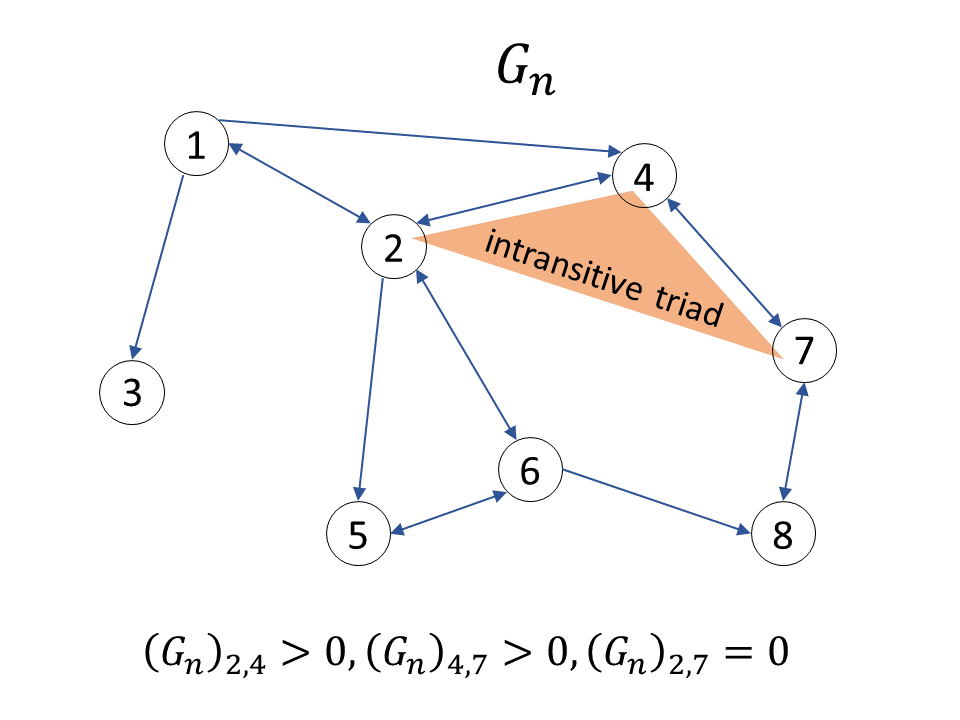
\includegraphics[width = 9cm]{intransitive.png}
		\caption{Intransitive triad}
	\end{center}
	\end{figure}
\end{example}

\hrulefill
\begin{exercise}\upshape
	Prove that if $|\beta| < 1$ the matrix $I_n - \beta G_n$ is nonsingular. (Hint: use Lemma \ref{lem:neumann})
\end{exercise}
\begin{exercise}\upshape
Prove that all row-sums of $G_n^t$ for all $t = 0, 1, \ldots$ are one when there are no isolated individuals.
\end{exercise}


\section{Estimation}\label{sec:estimation_soc}

Let us recall that the model to be estimated is \eqref{eq:bramat}:
\[
	\mbf{Y}_n = \alpha_0 \mathbf{1}_n + \beta_0 G_n \mbf{Y}_n + \mbf{X}_n \gamma_0 +  G_n \mbf{X}_n \delta_0 + \mcl{E}_n,
\]
where $\theta_0$ is the true parameter value of $\theta = (\alpha, \beta, \gamma, \delta)$.
Given the identification results as above, we here provide an approach to estimate $\theta_0$
In this section, we do not restrict the dimension of $X$ to be one.

First of all, it should be clear that the OLS estimator that simply regresses $\mbf{Y}_n$ on $(\mathbf{1}_n, G_n \mbf{Y}_n, \mbf{X}_n, G_n \mbf{X}_n)$ is inconsistent because of the endogeneity of $G_n \mbf{Y}_n$; if $i$ and $j$ are friends such that $i \in P_j$,
\begin{align*}
	\E[Y_j \epsilon_i]
	& = \E\left[\left(\alpha +\frac{\beta_0}{ n(j)} \sum_{k \in P_j} Y_k + X_j^\top \gamma_0 + \frac{1}{n(j)} \sum_{k \in P_j} X_k^\top \delta_0 + \epsilon_j\right) \epsilon_i\right] \\
	& = \frac{\beta_0}{ n(j)} \underbrace{\E\left[ \sum_{k \in P_j} Y_k \epsilon_i\right]}_{\neq \: 0} + \E[\epsilon_j \epsilon_i ].
\end{align*}
Thus, even when $\epsilon_i$ and $\epsilon_j$ are uncorrelated, unless $\beta_0 = 0$, $\E[Y_j \epsilon_i] \neq 0$ in general.

To account for this endogeneity problem, we can use a 2SLS estimator with instrumental variables.
Fortunately, a set of reasonable instrumental variables for $G_n\mbf{Y}_n$ can be easily found.
Observe that
\[
	G_n \mbf{Y}_n = \alpha_0 G_n \mathbf{1}_n + \beta_0 G^2_n \mbf{Y}_n + G_n \mbf{X}_n \gamma_0 +  G^2_n \mbf{X}_n \delta_0 + G_n \mcl{E}_n.
\]
This expression implies that $G^2_n \mbf{X}_n$ is a valid instrument for $G_n\mbf{Y}_n$, which is not included in the outcome equation \eqref{eq:bramat}, and is correlated with $G_n\mbf{Y}_n$ (assuming that $\delta_0 \neq 0$) but not with $\mcl{E}_n$.\footnote{
	Note that if the matrices $I_n$, $G_n$, and $G_n^2$ are linearly dependent, $G^2_n \mbf{X}_n$ is perfectly collinear with $(\mbf{X}_n, G_n\mbf{X}_n)$, and thus $G^2_n \mbf{X}_n$ cannot be used as an identifying instrument.
	From this, one can view the identification condition in Proposition \ref{prop:bra} that $I_n$, $G_n$, and $G_n^2$ are linearly independent as a condition ensuring that $G^2_n \mbf{X}_n$ becomes a valid instrument for $G_n\mbf{Y}_n$.
}

The 2SLS estimation procedure is as follows.
First, run a least squares regression of $G_n \mbf{Y}_n$ on $\mbf{Z}_n = (\mbf{1}_n, \mbf{X}_n, G_n\mbf{X}_n, G_n^2\mbf{X}_n)$, and compute the predicted value of $G_n\mbf{Y}_n$, say $\hat{G_n\mbf{Y}_n}$, by
\[
\hat{G_n\mbf{Y}_n} = \mbf{Z}_n(\mbf{Z}_n^\top \mbf{Z}_n)^{-1}\mbf{Z}_n^\top G_n \mbf{Y}_n.
\]
In the second stage,  run a least squares regression of $\mbf{Y}_n$ on $(\mbf{1}_n, \hat{G_n\mbf{Y}_n}, \mbf{X}_n, G_n\mbf{X}_n)$ to obtain the estimator $\hat \theta_n$ of $\theta$.
Note that since $(\mbf{1}_n, \mbf{X}_n, G_n\mbf{X}_n)$ is a subset of $\mbf{Z}_n$, it holds that $(\mbf{1}_n, \mbf{X}_n, G_n\mbf{X}_n) = \mbf{Z}_n(\mbf{Z}_n^\top \mbf{Z}_n)^{-1}\mbf{Z}_n^\top (\mbf{1}_n, \mbf{X}_n, G_n\mbf{X}_n)$, and the second-stage regression is numerically equivalent to regressing $\mbf{Y}_n$ on $\mbf{Z}_n(\mbf{Z}_n^\top \mbf{Z}_n)^{-1}\mbf{Z}_n^\top \mbf{H}_n$, where $\mbf{H}_n = (\mbf{1}_n, G_n\mbf{Y}_n, \mbf{X}_n, G_n\mbf{X}_n)$.
Hence, the 2SLS estimator $\hat \theta_n$ can be obtained actually in one step by
\begin{align}\label{eq:2slssoc}
\hat \theta_n = \left[\mbf{H}_n^\top \mbf{Z}_n(\mbf{Z}_n^\top \mbf{Z}_n)^{-1}\mbf{Z}_n^\top \mbf{H}_n  \right]^{-1}\mbf{H}_n^\top \mbf{Z}_n(\mbf{Z}_n^\top \mbf{Z}_n)^{-1}\mbf{Z}_n^\top\mbf{Y}_n.
\end{align}
Under some regularity conditions, the 2SLS estimator $\hat \theta_n$ is consistent for $\theta_0$ and asymptotically normally distributed at $\sqrt{n}$ rate; see Section \ref{sec:2slsAsymptotics}.

%%%%%%%%%%%%%%%%%%%%%%%%%%%%%%%%%%%%%%%%%%%%%%%%%
%%%%%%%%%%%%%%%%%%%%%%%%%%%%%%%%%%%%%%%%%%%%%%%%%
%%%%%%%%%%%%%%%%%%%%%%%%%%%%%%%%%%%%%%%%%%%%%%%%%

\chapter{Spatial Data}\label{chap:spatial_correlation}

\section{Spatial data}

\textbf{Spatial data\index{spatial data}} are data that are related to geographic information as part of that data. 
Geographic information refers to all kind of data that identify the spatial location of each data unit, which is stored not only in the form of point data (i.e., longitude and latitude), but also in the form of spatial polygon data (e.g., regions, districts, and municipalities) and mesh data (e.g., the distribution of air pollutants, satellite images, and brain images).
\begin{figure}[h!]
	\begin{center}
		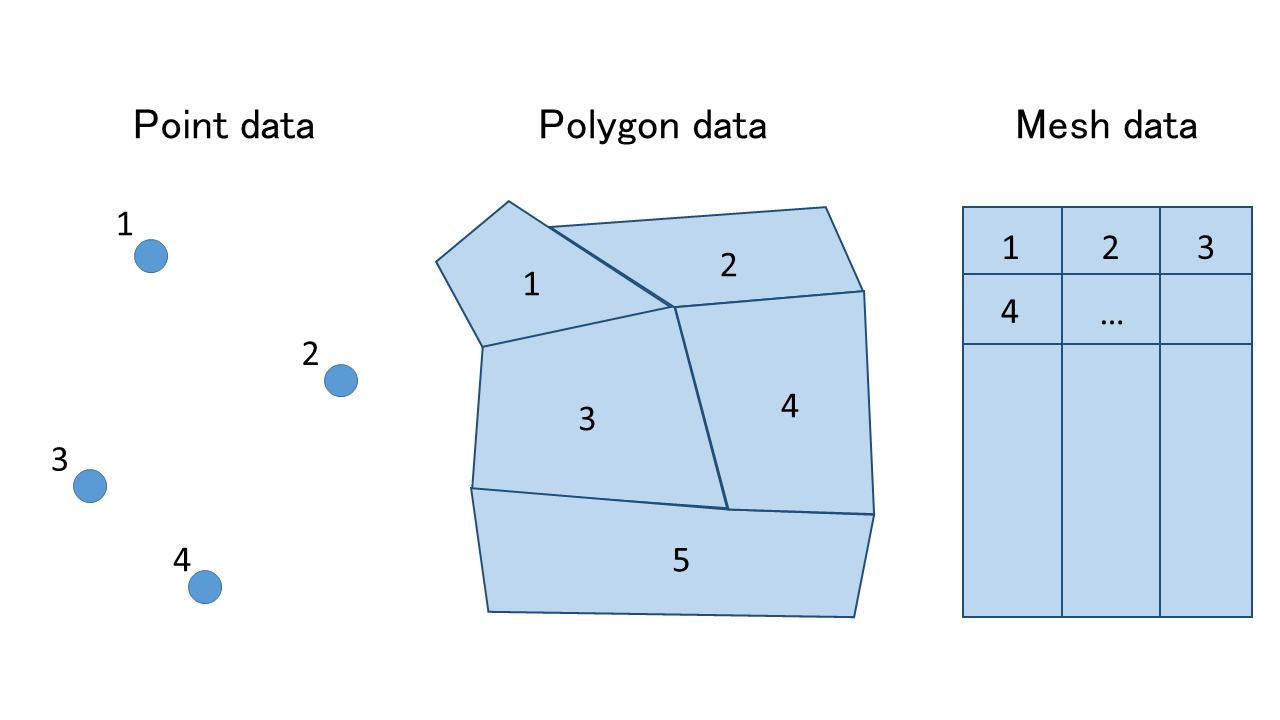
\includegraphics[width = 12cm]{spdata.png}
		\caption{Spatial data\label{fig:spdata}}
	\end{center}
\end{figure}

An integrated computational system, which is designed to store, manipulate, and visualize spatial data, is called \textbf{GIS\index{GIS}} (geographic information system). 
 The world's most popular GIS software is ArcGIS (ESRI).
 In these days, free and open source GIS softwares, such as QGIS and Grass GIS, have been becoming more popular.  
The statistical software \textbf{R} is also able to process and analyze spatial information with additional packages (such as \textbf{sf}, \textbf{spdep}, etc).

\begin{figure}[h!]
	\begin{center}
		
\includegraphics[width = 12cm]{GIS.png}
		\caption{Open-source free GIS\label{fig:GIS}}
	\end{center}
\end{figure}

\section{Moran's I and Geary's C}

\subsection{Spatial weight matrix}

The first step in any spatial data analysis is to plot the data on a map to find out if there is a specific correlational pattern in the data.
Figure \ref{fig:Tuberculosis} and \ref{fig:crime} are examples of plotted spatial data (polygon data).
In these examples, we can find a tendency that districts of similar values are spatially clustered.
This phenomenon is called \textbf{spatial autocorrelation\index{spatial autocorrelation}}, more precisely speaking, a ``positive'' spatial autocorrelation.
Negative spatial autocorrelation means that nearby districts have dissimilar values.
Although negative spatial autocorrelation is rarely observed in real data, a spatial competition under strategic substitutes potentially may generate a negative correlation (e.g., where to open convenience stores).
\begin{figure}[h!]
	\begin{center}
		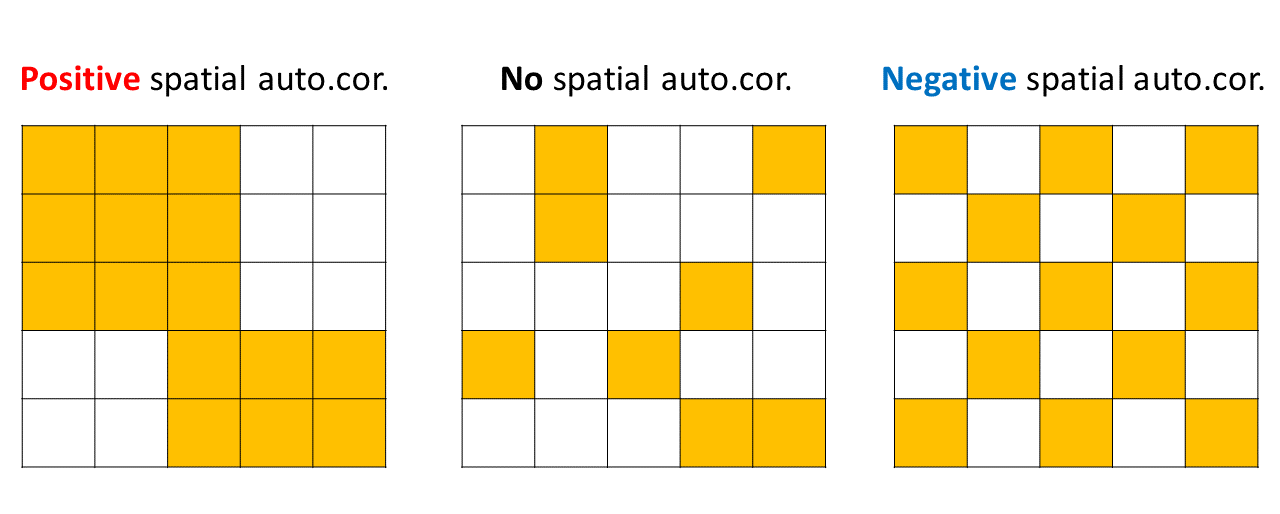
\includegraphics[width = 12cm]{spauto.png}
		\caption{Spatial autocorrelation}
	\end{center}
\end{figure}

The main objectives of spatial data analysis are to quantify and to analyze the mechanism of spatial autocorrelation in the data. 
In measuring the degree of spatial autocorrelation, one thing that needs clarification is what ``nearby'' means.
How to measure the proximity between two spatial units depends on the form of spatial data.
For point data, the proximity can be defined simply by the Euclidean distance (or, possibly other distance measures, such as road distance and travel time).
For polygon data, the proximity is often determined by whether the units share a common border or not.
For this type of proximity measure, there are two common approaches: \textbf{Rook contiguity\index{Rook contiguity}} and \textbf{Queen contiguity\index{Queen contiguity}} (based on the movement of chess pieces).
The rook contiguity defines neighbors by the existence of a common edge between two spatial units, and the queen contiguity is based on the existence of either a common edge or vertex between them (see Figure \ref{fig:contiguity}).
Note that, if one specifies a representative point of each polygon (e.g., location of administrative office, center of gravity), the distance-based proximity can be used for polygon data as well.

\begin{figure}[h!]
	\begin{center}
		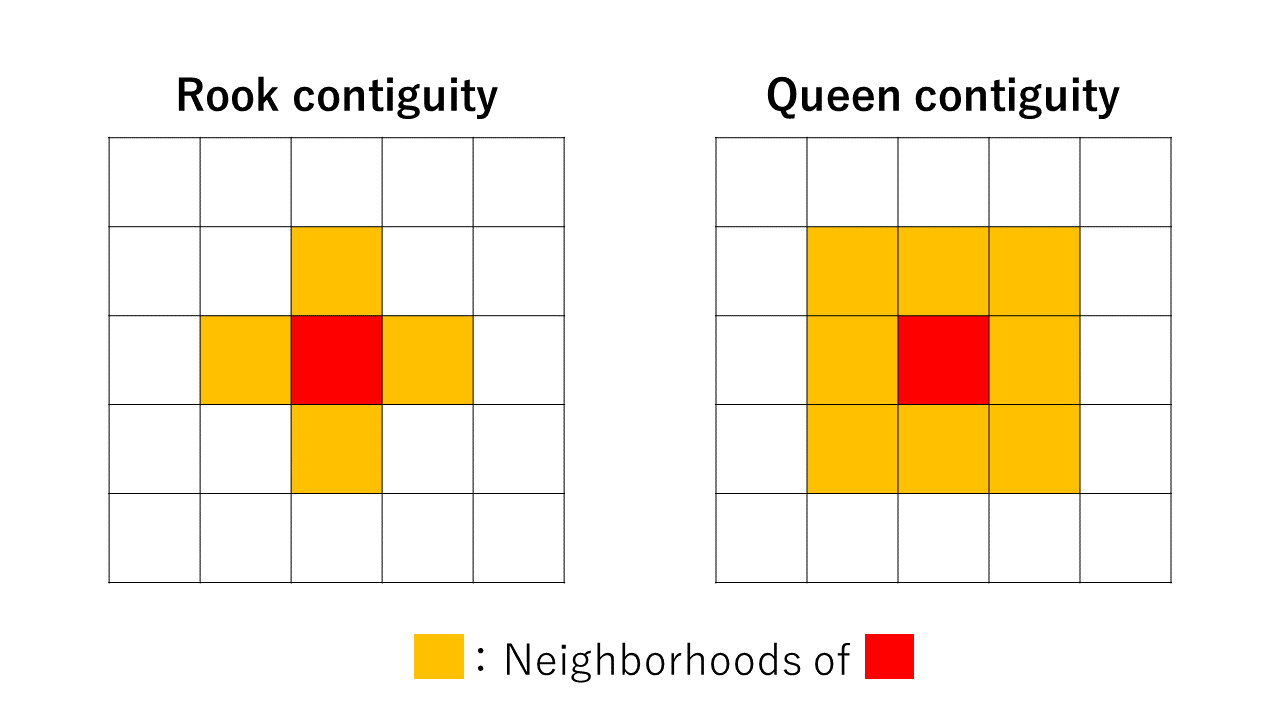
\includegraphics[width = 10cm]{adj.png}
		\caption{Rook contiguity and Queen contiguity\label{fig:contiguity}}
	\end{center}
\end{figure}

Now, consider a variable $X$, and suppose that we have sample data $\{X_1, \ldots, X_n\}$ of size $n$, where the subscript denotes each spatial unit.
Further, let $w_{ij}$ $(1 \le i,j \le n)$ be positive constants satisfying
\begin{align*}
\text{(i)} & \quad w_{ii} = 0  \;\; \text{for all $i$}\\
\text{(ii)} &\quad  w_{ij} \ge 0 \;\; \text{if $i$ and $j$ are close}\\
\text{(iii)} &\quad  w_{ij} = 0 \;\; \text{if $i$ and $j$ are distant enough}\\
\text{(iv)} &\quad  \sum_{j = 1}^n w_{ij} =1 \;\; \text{for all $i$}.
\end{align*} 
Such $w_{ij}$ is called the \textbf{spatial weight\index{spatial weight}} between $i$ and $j$.
Using the spatial weight, we can define the weighted ``neighborhood average'' of $X$ around unit $i$ by
\[
	X_i^* \equiv \sum_{j=1}^n w_{ij} X_j.
\]
Note that $i$ is not included in its own neighborhood ($w_{ii} = 0$).

\subsection*{Examples of spatial weights}
\paragraph{Polygon data}
In the case of polygon data, a commonly used spatial weight is as follows:
\[
	\begin{array}{ll}
	w_{ij} = \frac{1}{\text{\# of adjacent districts to $i$}}& \text{ if $j$ is adjacent to $i$} \\
	& \\
	w_{ij} = 0 &  \text{ if $j$ is not adjacent to $i$.} 
	\end{array}
\]
With this spatial weight, $X_i^*$ can be interpreted as the average of $X$ over the districts that are adjacent to $i$.
Note that the requirements $w_{ii} = 0$ and $\sum_{j = 1}^n w_{ij} =1$ for all $i$ means that there are no isolated districts, such as islands.
The latter condition is introduced for expositional simplicity, and can be relaxed in practice.

\paragraph{Point data}
In the case of point data, we first need to calculate the distance between every pair of spatial units, say $d(i,j)$.
Define,
\[
	\begin{array}{ll}
	v_{ij} = \frac{1}{d(i,j)^r}& \text{ if $d(i,j) \leq q $ and $j \neq i$} \\
	& \\
	v_{ij} = 0 &  \text{ otherwise } 
	\end{array}
\]
where $r$ is some positive number, which is typically 1 or 2, and $q$ is a pre-specified threshold value such that the objects with distance larger than $q$ are assumed to be independent.
Note that the $v_{ij}$'s defined above do not generally satisfy $\sum_{j = 1}^n v_{ij} = 1$.
Thus, we normalize them in the following way:
\[
	w_{ij} = \frac{v_{ij}}{\sum_{j' = 1}^n v_{ij'}}.
\]
This type of spatial weight is often called the distance-based spatial weight.
\bigskip

An $n \times n$ matrix $W_n$ whose $(i,j)$-th entry is given by $w_{ij}$ is called the \textbf{spatial weight matrix\index{spatial weight matrix}}: namely,
\[
	W_n = \left(\begin{array}{cccc}
		0            & w_{12} & \cdots & w_{1n} \\
		w_{21} &  0           & \cdots & w_{2n} \\
		\vdots    & \vdots    & \ddots & \vdots \\
		w_{n1} & w_{n2} & \cdots & 0
		\end{array}\right)
\]
One can view that the spatial weight matrix $W_n$ is a spatial version of the weighted social interaction matrix $G_n$.
Note that $W_n$ is not necessarily a symmetric matrix.
Using the spatial weight matrix, we can simply write $(X^*_1, \ldots, X_n^*)^\top = W_n \mbf{X}_n$, where  $\mbf{X}_n = (X_1, \ldots, X_n)^\top$.
\bigskip

Now, we are ready to more formally describe the definition of spatial autocorrelation.
We say that there exists a positive (resp. negative) spatial autocorrelation in the data if $\mbf{X}_n$ and $W_n \mbf{X}_n$ are positively (resp. negatively) correlated.
As one may notice, the determination of the existence of spatial autocorrelation is dependent and sensitive to the (somewhat arbitrarily) chosen spatial weights matrix $W_n$.

\subsection{Moran's I and Geary's C}

There are two major statistics to measure the magnitude of spatial autocorrelation.
The one is \textbf{Moran's I\index{Moran's I}} statistic, and the other is \textbf{Geary's C\index{Geary's C}} statistic, which are defined by
\[
	I \equiv \frac{\sum_{i=1}^n \sum_{j = 1}^n w_{ij}(X_i - \bar{X}_n) (X_j - \bar{X}_n)}{\sum_{i=1}^n (X_i - \bar{X}_n)^2}
\]
and
\[
	C \equiv \frac{n - 1}{2 n} \frac{\sum_{i=1}^n \sum_{j = 1}^n w_{ij}(X_i - X_j )^2}{\sum_{i=1}^n (X_i - \bar{X}_n)^2}
\]
respectively, where $\bar X_n = n^{-1}\sum_{i=1}^n X_i$.
Since Moran's I is a spatial extension of the standard (i.e., Pearson's) correlation coefficient between $\mbf{X}_n$ and $W_n \mbf{X}_n$, $I$ takes the value on the range $[-1, 1]$:
\[
\begin{array}{ll}
	\;\;\;0 < I \le 1 & \text{Positive spatial autocorrelation} \\
	\;\;\;\;\;\; I = 0 & \text{No spatial autocorrelation} \\
	-1 \leq I < 0 & \text{Negative spatial autocorrelation.}
\end{array}
\]
On the other hand, Geary's C ranges in value from $0$ to $2$, and the degree of spatial autocorrelation decreases as $C$ increases:
\[
\begin{array}{lc}
	1 < C \le 2 & \text{Negative spatial autocorrelation} \\
	\;\;\; C = 1 & \text{No spatial autocorrelation} \\
	0 \leq C < 1 & \text{Positive spatial autocorrelation.}
\end{array}
\]

Figure \ref{fig:IandC} provides numerical examples of Moran's I and Geary's C statistic based on the rook contiguity-based spatial weight.
\begin{figure}[h!]
	\begin{center}
		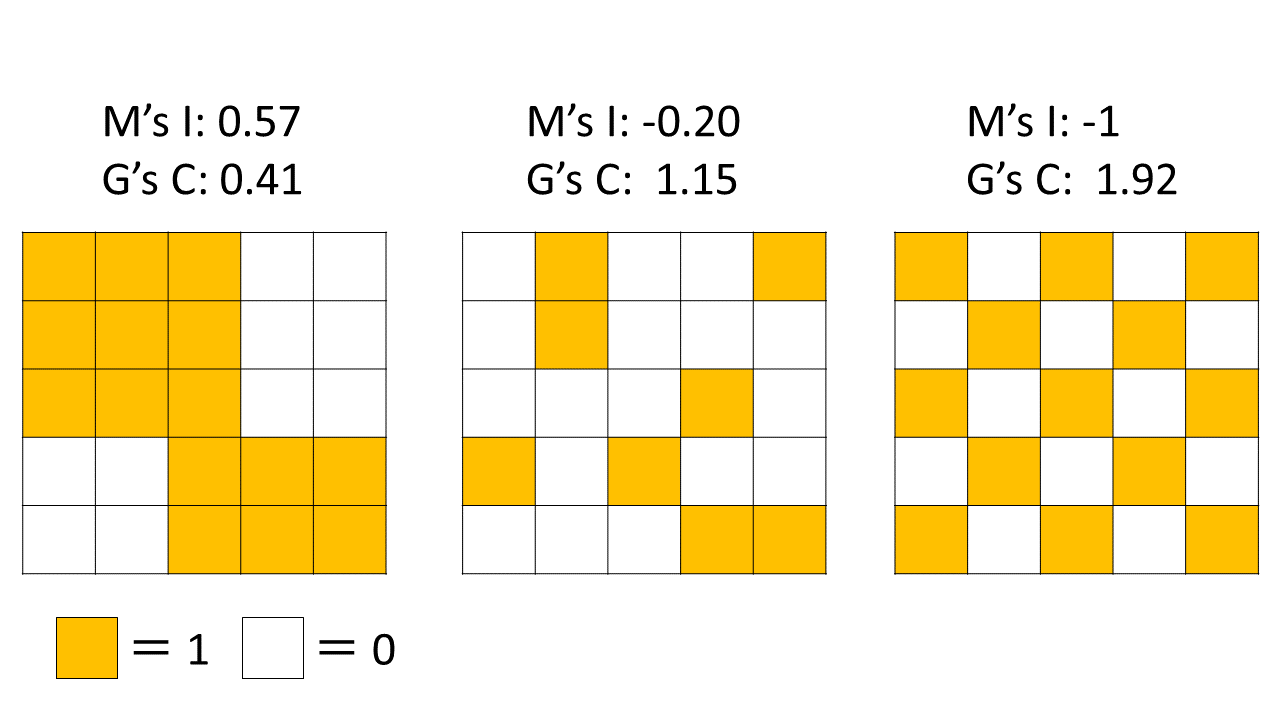
\includegraphics[width = 12cm]{IandC.png}
		\caption{Numerical examples: Moran's I and Geary's C\label{fig:IandC}}
	\end{center}
\end{figure}

\section{Spatial random variables}
\subsection{Spatial stochastic process}
In applications, it is mostly the case that $X$ is a random variable rather than a non-stochastic variable.
Suppose that each realized value of $X$ is uniquely characterized by its location $s$ in $\mathbb{R}^2$, and we may write $X \equiv X(s)$.
The collection of random variables $\{X(s) : s \in \mcl{S}_n\}$ is called as a \textbf{spatial stochastic process\index{spatial stochastic process}} (random field) with the sampling region $\mcl{S}_n \subseteq \mathbb{R}^2$.
The sampling region $\mcl{S}_n$ can be dependent on the sample size $n$, and it is usually required that $\mcl{S}_n$ expands as $n$ increases in each direction in $\mathbb{R}^2$, as stated below.

If $X(s)$ is independent of $X(s')$ for all $s \neq s'$, a random sample $\{X_1, \ldots, X_n\}$ of $X$ from $n$ distinct locations $\{s_i \in \mcl{S}_n: 1 \le i \le n\}$, where $X_i \equiv X(s_i)$, can be virtually treated as the standard non-spatial data.
In this case, letting $\sigma^2(s) = \Var(X(s)) < \infty$, we have
\[
	\Var\left( \bar X_n\right) = \frac{1}{n} \bar{\sigma}^2_n \to 0,
\]
as $n \to \infty$, where $\bar{\sigma}^2_n = \frac{1}{n}\sum_{i=1}^n \sigma^2(s_i)$.
Thus, by Chebyshev's inequality (\ref{eq:chevyshev}), for any positive constant $\kappa >0$,
\[
	\Pr\left( \left| \bar X_n - \E \bar X_n \right| \ge \kappa \right) \le \frac{\Var(\bar X_n)}{\kappa^2} \to 0,
\]
implying that the WLLN holds: $\bar X_n \overset{p}{\to} \E \bar X_n$. 
Similarly, it can be straightforwardly verified that the CLT also holds (under some additional regularity conditions).

However, the above argument is not realistic for spatial data in that $\{X_1, \ldots, X_n\}$ are independent.
It is clear that if the dependence between the variables is strong such that $\Var\left( \bar X_n\right)$ does not converge to zero, standard large sample theory would not be applicable.
In contrast, even when they are dependent, it is possible to show that the law of large numbers and the central limit theorem hold only if the degree of dependence is sufficiently weak.

Here, for simplicity, assume that the data points are located on a regular lattice in $\mathbb{R}^2$, and that $\Cov(X(s), X(s')) \equiv C(s, s') = \rho$, where $0 < \rho < \infty$, if $(s, s')$ are neighboring grid-points, and $C(s, s') = 0$ otherwise.

\begin{figure}[h!]
	\begin{center}
		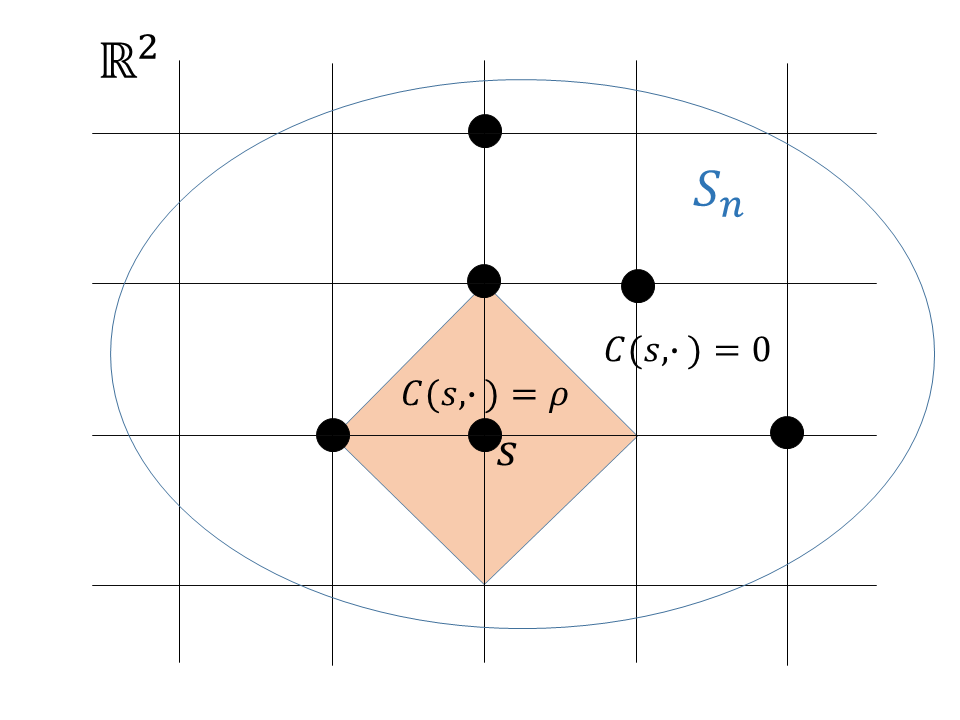
\includegraphics[width = 9cm]{sprnd.png}
		\caption{A type of weak spatial dependence}
	\end{center}
\end{figure}

The assumption that the covariance between the variables at two different locations depends only on the distance between them is called \textbf{isotropy\index{isotropy}} (i.e., directions do not matter).

Then, noting that there are at most four neighboring data points for each $s$, we have
\begin{align*}
	\Var(\bar X_n) 
	& = \frac{1}{n^2}\sum_{i=1}^n \sigma^2(s_i) + \frac{1}{n^2}\sum_{i = 1}^n \underbrace{\sum_{j \neq i}^n C(s_i, s_j)}_{\le \: 4\rho} \\
	& \le \frac{1}{n}\bar{\sigma}_n^2 + \frac{1}{n} 4 \rho \to 0
\end{align*}
as $n \to \infty$.
Therefore, the WLLN holds, and so does CLT with some weak additional conditions.
Although the spatial dependence structure introduced in this example is too simplistic for real data, more realistic dependence structures are proposed in the literature, for example, \textit{spatial mixing} and \textit{spatial near epoch dependence}, which are both natural spatial extensions of the dependence concept used in time series analysis.

\subsection{Spatial sampling}
 
 As mentioned above, if the degree of spatial dependence is sufficiently weak, one can rely on standard large sample theory.
It is important to note that such assumption implicitly requires that the sampling region must be (weakly) expanding: $\mcl{S}_n \subseteq \mcl{S}_{n + 1} \subseteq \cdots \subseteq \mbb{R}^2$, with the minimum distance between observations being fixed away from zero.
Large sample theory based on this type of data sampling framework is called \textbf{increasing domain asymptotics\index{increasing domain asymptotics}}.

On the other hand, suppose that the sampling region is fixed and bounded:  $\mcl{S}_n = \mcl{S}_{n + 1}  = \cdots \subset \mbb{R}^2$.
In this case, as the sample size $n$ increases, the observations get denser and denser.
Consequently, for a given data point $s$, the number of observations that are spatially dependent of $s$ can increase to infinity as $n$ increases.
This case is called \textbf{infill asymptotics\index{infill asymptotics}} (or fixed domain asymptotics).
As can be easily imagined, asymptotic theory under the infill asymptotics is much more involved than the one under the increasing domain asymptotics.
The infill asymptotic theory has been an important research field particularly in the literature on high frequency time series.

\begin{figure}[h!]
	\begin{center}
		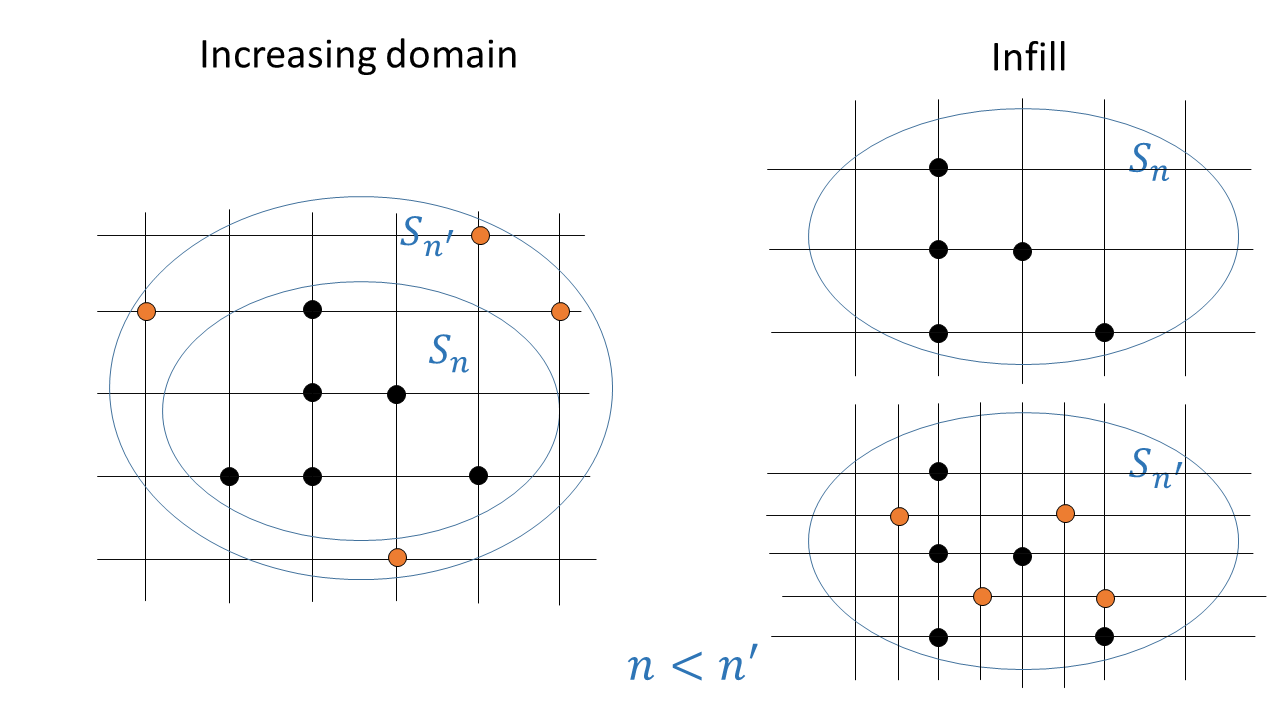
\includegraphics[width = 12cm]{asymptotics.png}
		\caption{Increasing domain asymptotics and infill asymptotics}
	\end{center}
\end{figure}
%%%%%%%%%%%%%%%%%%%%%%%%%%%%%%%%%%%%%%%%%%%%%%%%%

\chapter{Spatial Econometrics}\label{chap:spatial_econometrics}

Spatial econometrics is a subfield of econometrics that deals with spatial interaction (spatial autocorrelation) across spatial units.
Spatial econometric tools have become popular as empirical data analysis techniques for a range of diverse topics, including local economic growth, property markets, local competition between municipalities, local crime, and so forth. 
There are two most commonly used spatial econometric models: the \textbf{spatial lag model\index{spatial lag model}} (or spatial autoregressive model) and the \textbf{spatial error model\index{spatial error model}}.
In terms of the three types of social interaction effects classified by \cite{manski1993identification}, the spatial lag model is a model that accounts for possible endogeneity of spatial interaction, and the spatial error model accounts for the spatially correlated effects.

\section{Spatial lag model}\label{sec:SLM}

Let $Y$ be a dependent variable of interest, and $X$ be the vector of explanatory variables including a constant term.
Suppose that a sample $\{(Y_i,X_i): 1 \le i \le n\}$ of size $n$ is observed.
Further, let $w_{ij}$ be a spatial weight term between $i$ and $j$.
Recall that $w_{ii} = 0$ for normalization.
Then, the following model is called the \textbf{spatial lag model\index{spatial lag model}} (SLM):
\begin{align}\label{eq:slm}
	Y_i = \rho_0 \sum_{j = 1}^n w_{ij} Y_j + X_i^\tr\beta_0 + \eps_i, \;\; i = 1,\ldots,n.
\end{align}
Here, $\rho_0$ is a parameter that captures the spatial endogenous effect, $\beta_0$ is a vector of unknown coefficients, and $\eps$ is an unobserved random variable such that $\E \eps = 0$.
The SLM assumes that the average outcome of the neighboring districts influences on own outcome.

For example, imagine that there are two districts, which are almost identical in terms of sociodemographic and economic characteristics.
Suppose that one of them is surrounded by areas with higher crime rates, and the other is  located in a low crime rate area.
Then, if the crime rate of the former district is higher than that of the latter, this suggests the existence of spatial endogenous effect, and the spatial parameter $\rho_0$ will be estimated as positive.

Let $W_n = (w_{ij})_{i,j = 1}^n$ be the spatial weight matrix, and write $\mbf{Y}_n = (Y_1, \ldots, Y_n)^\top$,$\mbf{X}_n = (X_1, \ldots , X_n)^\top$,and $\mcl{E}_n = (\eps_1, ...., \eps_n)^\top$.
Then, we can rewrite model \eqref{eq:slm} in matrix form as
\[
	\mbf{Y}_n =  \rho_0 W_n \mbf{Y}_n + \mbf{X}_n \beta_0 + \mcl{E}_n.
\]
As one can see, the form of the SLM is quite similar to that of the social interaction model in \eqref{eq:bramat}.
Indeed, the SLM can be interpreted in the same manner as in the social interaction model.
That is, the SLM can be viewed as a game model of complete information with the realized outcomes $\{Y_1, \ldots, Y_n \}$ being a result of Nash equilibrium behavior.\footnote{
	In this case, the source of spatial autocorrelation is the presence of local strategic interaction.
	However, in many applications, what mechanisms generate the spatial autocorrelation is less concerned, and researchers often introduce a model like \eqref{eq:slm} a priori.
}
In addition, if $|\rho_0| < 1$ and the spatial weight matrix is normalized such that each row sums to unity, the matrix $I_n - \rho_0 W_n$ is nonsingular, and thus the inverse matrix 
$(I_n - \rho_0 W_n)^{-1}$ exists.
Thus, the reduced-form of the SLM can be obtained by
\[
	\mbf{Y}_n =  (I_n - \rho_0 W_n)^{-1}\mbf{X}_n \beta_0 + (I_n - \rho_0 W_n)^{-1}\mcl{E}_n.
\]

By Neumann series expansion (Appendix \ref{sec:neumann}), we have 
\[
	(I_n - \rho_0 W_n)^{-1}\mbf{X}_n\beta_0 = \mbf{X}_n\beta_0 + \rho_0 W_n \mbf{X}_n\beta_0 + \rho_0^2 W_n^2\mbf{X}_n\beta_0 + \cdots.
\]
Similarly to the social interaction model, the second term on the right-hand side represents the effect of the neighbors' characteristics, and the third term is the effect from the neighbors' neighbors' characteristics, and so forth.
This implies that a marginal increase in $X$ affects not only own outcome $Y$ but the outcomes of the others, and vice versa.
In the context of spatial econometrics, the matrix $(I_n - \rho_0 W_n)^{-1} $ is called the \textbf{spatial multiplier} matrix.

\subsection{Maximum likelihood estimation}

 For the same reason mentioned in Section \ref{sec:estimation_soc}, a simple OLS estimator that regresses $\mbf{Y}_n$ on $(W_n \mbf{Y}_n, \mbf{X}_n)$ is not consistent because of the endogeneity of $W_n \mbf{Y}_n$.
 To deal with this problem, one may use a maximum likelihood approach.
 Specifically, assume that the error terms $(\eps_1, \ldots , \eps_n)$ are IID as normal $N(0, \sigma_0^2)$.
 Then, the conditional joint distribution of $\mbf{Y}_n$ given $\mbf{X}_n$ is characterized by
 \[
 	\mbf{Y}_n \mid \mbf{X}_n \sim \mbf{N}\left( (I_n - \rho_0 W_n)^{-1}\mbf{X}_n \beta_0, \; (I_n - \rho_0 W_n)^{-1}(I_n - \rho_0 W_n^\top)^{-1}\sigma_0^2\right),
 \]
and one can show that the log-likelihood function of the SLM is given by
\begin{align*}
 	\ell^{SLM}_n(\rho, \beta, \sigma^2) 
 	&= -\frac{n}{2} \log (2\pi) -\frac{n}{2} \log\sigma^2 + \log | I_n - \rho W_n| \\
 	& \quad - \frac{1}{2\sigma^2} ((I_n - \rho W_n)\mbf{Y}_n - \mbf{X}_n \beta)^\top ((I_n - \rho W_n)\mbf{Y}_n - \mbf{X}_n \beta),
 \end{align*}
where $|A_n|$ denotes the determinant of the matrix $A_n$.
Then, we can obtain a consistent estimator of $(\rho_0, \beta_0, \sigma_0^2)$ as the maximizer of the above log-likelihood function; see \cite{lee2004asymptotic} for details on the theoretical properties of this estimator.

However, this maximum likelihood estimation has two serious drawbacks.
First, the assumption that $(\eps_1, \ldots , \eps_n)$ are IID normal is very restrictive for spatial data, since spatial units are naturally correlated and heterogeneous in several characteristics, such as area size and population.
Second, the computation of the objective function $\ell^{SLM}_n(\rho, \beta, \sigma^2)$ can be quite expensive when the sample size is not small; calculating the determinant of a large matrix is very time-consuming and often computationally intractable.
Fortunately, as described below, one can obtain a consistent estimator of the model parameters by the 2SLS method of \cite{kelejian1998generalized}, without relying on the IID normality assumption.

\subsection{2SLS estimation}\label{subsec:2sls}

To simplify the exposition, in the following we assume that the regressor $X$ is non-stochastic and bounded in absolute value.\footnote{
	The assumption of non-stochastic regressors is often adopted in the literature of spatial econometrics, partly for the purpose of avoiding tedious technical discussions on the underlying spatial random process.
	In the non-stochastic regressors framework, we should interpret the analysis as being conditional on the realization of these variables.
}
Then, since $\E \eps  = 0$, this automatically implies that the regressor $X$ is exogenous: $\E[X\eps] = X \E[\eps] = 0$.

Suppose that the matrix $I_n - \rho_0 W_n$ is nonsingular with $|\rho_0| < 1$.
Then, we have
\begin{align*}
	W_n \mbf{Y}_n 
	& = W_n(I_n - \rho_0 W_n)^{-1}\mbf{X}_n\beta_0 + W_n (I_n - \rho_0 W_n)^{-1}\mcl{E}_n\\
	& = W_n\mbf{X}_n\beta_0 + \rho_0 W^2_n\mbf{X}_n\beta_0 + \rho^2_0 W^3_n\mbf{X}_n\beta_0 + \cdots +  W_n (I_n - \rho_0 W_n)^{-1}\mcl{E}_n.
\end{align*}
The first line implies that the ideal instrumental variable for the endogenous regressor $W_n\mbf{Y}_n$ is $W_n(I_n - \rho W_n)^{-1}\mbf{X}_n\beta$.
However, we cannot use this since $\rho_0$ and $\beta_0$ are unknown in practice.
The second line shows that the ideal instrument $W_n(I_n - \rho_0 W_n)^{-1}\mbf{X}_n\beta_0$ is expressed as a linear combination of $\{W_n\mbf{X}_n, W^2_n\mbf{X}_n, \ldots\}$.
Thus, a subset of columns of $\{W_n\mbf{X}_n, W^2_n\mbf{X}_n, \ldots\}$ can be used as a feasible and reasonable instrument for $W_n\mbf{Y}_n$.
Specifically, let $\mbf{Z}_{n1}$ be a matrix of instrumental variables composed of a subset of linearly independent columns of $\{W_n\mbf{X}_n, W^2_n\mbf{X}_n, \ldots\}$, and define $\mbf{Z}_n = (\mbf{X}_n, \mbf{Z}_{n1})$.
Then, a consistent estimator of $\theta_0 = (\rho_0, \beta_0^\top)^\top$ can be obtained the 2SLS method as follows.
In the first step, we regress the endogenous variable $W_n \mbf{Y}_n$ on $\mbf{Z}_n$, and obtain the predicted value of $W_n\mbf{Y}_n$ by 
\[
	\hat{W_n\mbf{Y}_n} = \mbf{Z}_n(\mbf{Z}_n^\top \mbf{Z}_n)^{-1}\mbf{Z}_n^\top W_n \mbf{Y}_n.
\]
In the second step, $\theta$ is estimated by a linear regression of $\mbf{Y}_n$ on $(\hat{W_n\mbf{Y}_n}, \mbf{X}_n)$.
Let $\hat \theta_n$ be the resulting estimator of $\theta_0$.
In the same manner as in \eqref{eq:2slssoc}, we can derive the closed-form expression for the 2SLS estimator $\hat \theta_n$ as
\begin{align}\label{eq:2sls}
	\hat \theta_n = \left[\mbf{H}_n^\top \mbf{Z}_n(\mbf{Z}_n^\top \mbf{Z}_n)^{-1}\mbf{Z}_n^\top \mbf{H}_n  \right]^{-1}\mbf{H}_n^\top \mbf{Z}_n(\mbf{Z}_n^\top \mbf{Z}_n)^{-1}\mbf{Z}_n^\top\mbf{Y}_n,
\end{align}
 where $\mbf{H}_n = (W_n\mbf{Y}_n, \mbf{X}_n)$. 
Asymptotic properties of the 2SLS estimator \eqref{eq:2sls} can be derived in the same way as in Section \ref{sec:2slsAsymptotics}.

\section{Spatial error model}\label{sec:SEM}

It is highly possible that the unobserved determinant of $Y$, $\eps$, involves some spatial factors.
If they are spatially correlated, the model has spatial correlated effects.
To account for the spatial correlated effects (i.e., spatial autocorrelation of $\eps$), we can consider the following model:
\begin{align}\label{eq:sem}
\begin{split}
	Y_i  & = X_i^\tr\beta_0 + \eps_i \\
	\eps_i & = \lambda_0 \sum_{j = 1}^n w_{ij} \eps_j + u_i, \;\; i = 1,\ldots,n
\end{split}
\end{align}
where $u_i$ is an idiosyncratic (non-spatial) error term such that $\E u = 0$, and $\lambda_0$ is the parameter that captures the spatial correlated effect.
The above model is called the \textbf{spatial error model\index{spatial error model}} (SEM).
In contrast to the SLM, the SEM does not admit the existence of spatial multiplier effects; that is, in SEM, an increase in own $X$ solely influences on own $Y$ and not on the others' outcomes.
Thus, these two models have quite different policy implications.

\subsection{Maximum likelihood estimation}
Again, we retain the assumption that $X$ is non-stochastic.
When the matrix $I_n - \lambda_0 W_n$  is nonsingular with $|\lambda_0| < 1$, the SEM can be re-written in matrix form as
\[
	\mbf{Y}_n =  \mbf{X}_n \beta_0 + (I_n - \lambda_0 W_n)^{-1}U_n,
\]
where $U_n = (u_1, \ldots, u_n)^\top$.
Then, since each $\eps$ can be expressed as a linear combination of $(u_1, \ldots, u_n)$, we have $\E \eps = 0$, and thus $\E[X \eps] = 0$ holds; that is, $X$ is exogenous.
Therefore, for the estimation of SEM, a simple OLS regression yields a consistent estimate of $\beta_0$, although not efficient and uninformative for the spatial parameter $\lambda_0$.

In order to estimate $\lambda_0$, we can consider a maximum likelihood estimation.
Assuming now that $(u_1, \ldots , u_n)$ are IID as normal $N(0, \sigma_0^2)$, the conditional joint distribution of $\mbf{Y}_n$  given $\mbf{X}_n$ is characterized by
\[
	\mbf{Y}_n \mid \mbf{X}_n \sim \mbf{N}\left(\mbf{X}_n \beta_0, \; (I_n - \lambda_0 W_n)^{-1}(I_n - \lambda_0 W_n^\top)^{-1}\sigma^2_0 \right).
\]
After some calculations, the log-likelihood function of the SEM can be obtained as follows:
\begin{align*}
	\ell^{SE}_n(\lambda, \beta, \sigma^2) 
	& = -\frac{n}{2} \log (2\pi) -\frac{n}{2} \log\sigma^2 + \log | I_n - \lambda W_n| \\
	& \quad - \frac{1}{2\sigma^2} (\mbf{Y}_n - \mbf{X}_n \beta)^\tr(I_n - \lambda W_n)^\tr (I_n - \lambda W_n) (\mbf{Y}_n  - \mbf{X}_n \beta).
\end{align*}
By maximizing the above log-likelihood function, we can obtain a consistent estimator of $(\lambda_0, \beta_0, \sigma^2_0)$.
However, the IID normality assumption is restrictive as mentioned above.
Also, again since the log-likelihood function involves the determinant of the matrix $I_n - \lambda W_n$, there can be significant difficulties in the practical computation of this estimator.
In order to overcome this issue, \cite{kelejian1999generalized} developed a method of moments (MM) estimator that is not dependent on the IID normality assumption and is computationally easy irrespective of the size of the sample.

\subsection{Method of moments estimation}\label{subsec:mm}

The estimation procedure of the MM estimator is implemented in two steps.
The first step estimates the coefficients $\beta_0$ by the OLS regression of $\mbf{Y}_n$ on $\mbf{X}_n$, and let $\hat \beta_n$ be the resulting estimator.
Here, we assume that $(u_1, \ldots , u_n)$ are homoskedastic with variance $\E[u_i^2] = \sigma_0^2$ for all $i$.\footnote{
	The homoskedasticity assumption is introduced for simplicity.
	A heteroskedasticity-robust version of the estimation procedure is explained in \cite{kelejian2010specification}.
}
In the second step, we estimate $(\lambda_0, \sigma_0^2)$ by the MM approach.
The estimator is based on the following three moment equalities: 
\begin{align*}
	\E\left[ U_n^\top U_n /n \right] = \sigma_0^2, \;\; \E\left[ \bar U_n^\top \bar U_n /n \right] =  \sigma_0^2  \mrm{trace}\left\{ W_n^\top W_n/n \right\}, \;\;  \E\left[ \bar U_n^\top U_n/n \right] = 0,
\end{align*}
where $\bar U_n = W_n U_n$.
Note that for any $n \times 1$ vectors $A_n$ and $B_n$, $A_n^\top B_n = \mrm{trace}\{ A_n B_n^\top \}$.
In the third equality, we have used the fact that the diagonal elements of $W_n$ are zero.
Let $\bar{\mcl{E}}_n = W_n \mcl{E}_n$ and $\bar{\bar{\mcl{E}}}_n = W_n W_n \mcl{E}_n$.
Since we have
\[
	U_n = \mcl{E}_n - \lambda_0 \bar{\mcl{E}}_n\; \text{ and }\; \bar U_n = \bar{\mcl{E}}_n - \lambda_0 \bar{\bar{\mcl{E}}}_n,
\]
 the above three equalities can be rewritten in terms of $\mcl{E}_n$ as
\begin{align*}\renewcommand{\arraystretch}{1.8}
\begin{array}{lllll}
	\E\left[ \mcl{E}_n^\top \mcl{E}_n /n\right] 
	& - 2\lambda_0 \E\left[ \mcl{E}_n^\top \bar{\mcl{E}}_n/n \right] 
	& +  \lambda^2_0 \E\left[ \bar{\mcl{E}}_n^\top \bar{\mcl{E}}_n/n \right] 
	& - \sigma^2_0 
	& = 0,\\
	\E\left[ \bar{\mcl{E}}_n^\top \bar{\mcl{E}}_n/n \right] 
	& - 2\lambda_0 \E\left[ \bar{\mcl{E}}_n^\top \bar{\bar{\mcl{E}}}_n/n \right] 
	& +  \lambda^2_0 \E\left[ \bar{\bar{\mcl{E}}}_n^\top \bar{\bar{\mcl{E}}}_n/n \right] 
	& - \sigma^2_0 \mrm{trace}\left\{ W_n^\top W_n/n \right\} 
	& = 0, \\
	\E\left[ \bar{\mcl{E}}_n^\top \mcl{E}_n/n \right] 
	& - \lambda_0 \E\left[ \bar{\mcl{E}}_n^\top \bar{\mcl{E}}_n/n + \bar{\bar{\mcl{E}}}_n^\top \mcl{E}_n/n\right] 
	& +  \lambda^2_0 \E\left[ \bar{\mcl{E}}_n^\top \bar{\bar{\mcl{E}}}_n/n \right]  
	&
	& = 0.
\end{array}
\end{align*}
Equivalently,
\begin{align*}
	\Gamma_n (\lambda_0, \lambda_0^2, \sigma_0^2)^\top - \gamma_n = \mbf{0},
\end{align*}
where
\[\renewcommand{\arraystretch}{1.8}
	\Gamma_n \equiv \left(
	\begin{array}{ccc}
	2 \E\left[ \mcl{E}_n^\top \bar{\mcl{E}}_n/n \right] 
	& - \E\left[ \bar{\mcl{E}}_n^\top \bar{\mcl{E}}_n/n \right] 
	& 1 \\
	2 \E\left[ \bar{\mcl{E}}_n^\top \bar{\bar{\mcl{E}}}_n/n \right] 
	& - \E\left[ \bar{\bar{\mcl{E}}}_n^\top \bar{\bar{\mcl{E}}}_n/n \right] 
	& \mrm{trace}\left\{ W_n^\top W_n/n \right\}  \\
	\E\left[ \bar{\mcl{E}}_n^\top \bar{\mcl{E}}_n/n + \bar{\bar{\mcl{E}}}_n^\top \mcl{E}_n/n\right] 
	& - \E\left[ \bar{\mcl{E}}_n^\top \bar{\bar{\mcl{E}}}_n/n \right]  
	& 0
	\end{array}
	\right)
	\qquad
	\gamma_n \equiv \left(\begin{array}{c}
	\E\left[ \mcl{E}_n^\top \mcl{E}_n /n\right] \\
	\E\left[ \bar{\mcl{E}}_n^\top \bar{\mcl{E}}_n/n \right] \\
	\E\left[ \bar{\mcl{E}}_n^\top \mcl{E}_n/n \right]
	\end{array}
	\right).
\]\renewcommand{\arraystretch}{1}
Thus, the true value of $(\lambda, \sigma^2)$ can be characterized as the minimizer of the objective function $|| \Gamma_n (\lambda, \lambda^2, \sigma^2)^\top - \gamma_n ||^2$, where $|| \cdot ||$ denotes the Euclidean norm.
This implies that we can estimate $(\lambda_0, \sigma^2_0)$ by minimizing the sample analog of $|| \Gamma_n (\lambda, \lambda^2, \sigma^2)^\top - \gamma_n ||^2$, where the expectations in the definition of $\Gamma_n$ and $\gamma_n$ are dropped, and $\mcl{E}_n$ is replaced by $\hat{\mcl{E}}_n = \mbf{Y}_n - \mbf{X}_n\hat \beta_n$.
Let the resulting MM estimator of  $(\lambda_0, \sigma^2_0)$ be $(\hat \lambda_n, \hat \sigma_n^2)$.
\cite{kelejian1999generalized} proved that the MM estimator $(\hat \lambda_n, \hat \sigma_n^2)$ is consistent under mild regularity conditions.
The limiting distribution of $(\hat \lambda_n, \hat \sigma_n^2)$ is complicated and is omitted here (see, e.g., \cite{kelejian2010specification}).
\bigskip

Once a consistent estimate $(\hat \lambda_n, \hat \sigma_n^2)$ is obtained, we can use a generalized least squares (GLS) estimator of $\beta_0$ to obtain a more efficient estimate.
Specifically, let
\[
	\hat \Omega_n \equiv (I_n - \hat \lambda_n W_n)^{-1}(I_n - \hat \lambda_n W_n^\top)^{-1} .
\]
Then, the GLS estimator of $\beta_0$ is defined by
\begin{align}\label{eq:gls}
	\hat \beta_n^{GLS} = \left[\mbf{X}_n^\top \hat \Omega_n^{-1} \mbf{X}_n \right]^{-1} \mbf{X}_n^\top \hat \Omega_n^{-1} \mbf{Y}_n.
\end{align}
The GLS estimator $\hat \beta_n^{GLS}$ is asymptotically efficient, with its covariance matrix being $ (\sigma^2/n)\left[\mbf{X}_n^\top \Omega_n^{-1} \mbf{X}_n / n \right]^{-1}$, where $\Omega_n \equiv (I_n - \lambda_0 W_n)^{-1}(I_n - \lambda_0 W_n^\top)^{-1}$.

\section{Empirical analysis with \textbf{R}: Household burglary in Tokyo}\label{sec:emp_burglar}

It is commonly observed that different locations sharing the same social and economic conditions do not necessarily experience the same crime intensity.
Instead, spatial clusters of crimes (i.e., ``hot spots'') exist.
Accordingly, it is important to incorporate spatial information in quantitative criminology research.
In this empirical analysis, we investigate the determinants of household burglary risk in Tokyo.

The dataset used here is the same as the one in \cite{hoshino2018semiparametric}.\footnote{
	The data files are available on request.
}
The variables used in the analysis are created from several data sources.
For crime data, we use the number of household burglaries recorded in 2011 by the Tokyo Metropolitan Police Department for each district in Tokyo.
The socio-demographic and economic information for each district are taken from the Census 2010 and the Commercial Statistics Survey 2009.
The definitions of the variables are summarized in the following table.
All variables are constructed at the district level.

\begin{center}
	\begin{tabular}{l|l|l}
		\multicolumn{3}{c}{ Variables and their definitions} \\ \hline\hline
				&  \multicolumn{1}{|c|}{\small Variable} &  \multicolumn{1}{|c}{\small Definition} \\ \hline
		\small Dependent variable & \small \textit{burglary} & ${\small 1,000\times }\dfrac{\text{{\small \# of recorded household burglaries}}}{\text{{\small \# of households}}}$ \\ 
		&  &  \\ 
		\small Explanatory variables & \small \textit{nhmem}  & \small Average number of household members. \\
													  & \small \textit{dnsty} & \small Residential density (\# of residences / Area of district). \\ 
		                                              & \small \textit{owner} & \small Portion of owner-occupied houses. \\
		                                              & \small \textit{elder}    & \small Portion of households headed by the elderly (over 65 years old). \\
		                                              & \small \textit{high}    & \small Portion of high-rise residential buildings. \\ 
		                                              & \small \textit{manag} & \small \# of workers in managerial positions / Labor force population. \\ 
		                                              & \small \textit{retail}      & \small Total area of retail stores in district / Area of district. \\ 
												     & \small Ward dummies & \small Dummies for the 23 special wards of Tokyo.$^\dagger$ \\ \hline
	\end{tabular}
	\begin{flushleft}
	($\dagger$: {\small Here, 22 dummy variables are introduced. Nerima ward is omitted as a benchmark.)}
	\end{flushleft}
\end{center}

After deleting the observations with missing values, a sample of $n = 3025$ observations is used in this analysis.
With this dataset, we estimate SLM \eqref{eq:slm} and SEM \eqref{eq:sem} by the 2SLS method and the MM method, respectively.
The spatial weight matrix is constructed based on Queen-contiguity and is row-normalized.

Set the \textbf{R} working directory appropriately, and read the csv files.
\begin{lstlisting}[basicstyle=\ttfamily\footnotesize, frame=single]
# Data #

 data <- as.data.frame(read.csv("TokyoCrime.csv"))
 n    <- nrow(data) # sample size (n = 3025)

# Spatial weight matrix #

 W <- as.matrix(read.csv("TokyoCrime_W.csv", header = FALSE))
\end{lstlisting}
The variables used are defined as follows.
\begin{lstlisting}[basicstyle=\ttfamily\footnotesize, frame=single]
# Variables #

 Y  <- data$burglary
 X1 <- with(data, cbind(nhmem, dnsty, owner, elder, high, manag, retail))

 ward23 <- as.numeric(data$ward)
 wdum   <- matrix(0, n, 22)
 for(i in 1:22) wdum[,i] <- ifelse(ward23 == i, 1, 0)

 X <- cbind(1, X1, wdum)
\end{lstlisting}

We first estimate the SLM.
In accordance with the notation in Section \ref{subsec:2sls}, define the variables as follows.
\begin{lstlisting}[basicstyle=\ttfamily\footnotesize, frame=single]
 H  <- cbind(W%*%Y, X)
 Z1 <- cbind(W%*%X1, W%*%W%*%X1, W%*%W%*%W%*%X1)
 Z  <- cbind(X, Z1)
\end{lstlisting}
As the instruments for $W_n \mbf{Y}_n$, we employ the first, second, and third-order spatial lags of the explanatory variables (excluding the constant and the ward dummies).
Then, following \eqref{eq:2sls}, we obtain the 2SLS estimate in the following manner.
\begin{lstlisting}[basicstyle=\ttfamily\footnotesize, frame=single]
# 2SLS estimation #

 P     <- Z%*%solve(t(Z)%*%Z)%*%t(Z)
 theta <- solve(t(H)%*%P%*%H)%*%t(H)%*%P%*%Y
\end{lstlisting}
We compute the covariance matrix of the 2SLS estimator under homoskedasticity.
Once the covariance matrix is obtained, we can then calculate the standard error and t-value of the estimated parameter.
\begin{lstlisting}[basicstyle=\ttfamily\footnotesize, frame=single]
# Covariance matrix under homoskedasticity #

 sigma2 <- mean((Y - H%*%theta)^2) 
 Q_ZZ   <- t(Z)%*%Z/n
 Q_ZH   <- t(Z)%*%H/n 
 Cov    <- (sigma2/n)*solve(t(Q_ZH)%*%solve(Q_ZZ)%*%Q_ZH)

 sd   <- diag(Cov)^0.5 # Standard error
 tval <- theta/sd      # t-value
\end{lstlisting}
The summary of the results is as follows. 
\begin{lstlisting}[basicstyle=\ttfamily\footnotesize, frame=single]
>  cbind(theta, sd, tval)
                     sd
        0.4257077087 0.18952982  2.246125184
        0.6074076919 0.23175842  2.620865663
nhmem  -0.1652634554 0.09324095 -1.772434221
dnsty   5.9766729090 3.18795297  1.874768216
owner   0.0733078500 0.16210661  0.452220004
elder   0.0625461529 0.35319744  0.177085524
high   -0.5562633330 0.12004293 -4.633870187
manag  -0.3134209803 0.92201410 -0.339930790
retail -0.4174281178 0.41219978 -1.012683981

== The results for the ward dummies are omitted to save space. ==
\end{lstlisting}
The results show that the spatial autocorrelation in the household burglary rate is positive and significant.
It indicates that a one-point increase in the average burglary rate of neighboring districts increases own district's burglary rate by about 0.4.
Among the other explanatory variables, we find that the \textit{high} variable significantly negatively affect the burglary rate.
This result would be a reflection of the fact that high-rise buildings are likely equipped with high-security system.
\bigskip

Next, we estimate the SEM.
The fist step of the estimation procedure is to estimate $\beta_0$ by OLS. 
\begin{lstlisting}[basicstyle=\ttfamily\footnotesize, frame=single]
# OLS estimation #

 beta <- lm(Y ~ X - 1)$coef
\end{lstlisting}
The second step is to implement the MM estimation.
In line with Section \ref{subsec:mm}, we define the following quantities.
\begin{lstlisting}[basicstyle=\ttfamily\footnotesize, frame=single]
 E  <- Y - X%*%beta
 E1 <- W%*%E
 E2 <- W%*%W%*%E

 Gam1 <- c(2*t(E)%*%E1/n,              -t(E1)%*%E1/n, 1)
 Gam2 <- c(2*t(E1)%*%E2/n,             -t(E2)%*%E2/n, sum(diag(t(W)%*%W))/n) 
 Gam3 <- c(t(E1)%*%E1/n + t(E2)%*%E/n, -t(E1)%*%E2/n, 0)
 Gam  <- rbind(Gam1, Gam2, Gam3)
 gam  <- c(t(E)%*%E/n, t(E1)%*%E1/n, t(E1)%*%E/n)
\end{lstlisting}
Then, the objective function to be minimized is defined as follows.
\begin{lstlisting}[basicstyle=\ttfamily\footnotesize, frame=single]
# Objective function in the MM estimation #

 ObjF <- function(param){

	g <- Gam%*%c(param[1], param[1]^2, param[2]^2) - gam
	sum(g^2)

	}
\end{lstlisting}
Here, the vector \texttt{param} is a 2-dimensional vector with its first element corresponding to the spatial parameter $\lambda$ and the second element to the standard error $\sigma$.
The minimizer of \texttt{ObjF} can be found by using the command \texttt{optim}.
To do this, we need to specify initial candidate values for $\lambda$ and $\sigma$, which are set to 0.5 and the standard deviation of the residuals (\texttt{sd(E)}), respectively.
\begin{lstlisting}[basicstyle=\ttfamily\footnotesize, frame=single]
 NLS    <- optim(c(0.5, sd(E)), ObjF)
 lambda <- NLS$par[1]
 sigma2 <- NLS$par[2]^2

>  c(lambda, sigma2)
[1] 0.1597388 0.9959481
\end{lstlisting}

Using these estimated values, we re-estimate $\beta_0$ by the GLS method.
Following \eqref{eq:gls}, the GLS estimate $\hat \beta_n^{GLS}$ is computed as follows.
\begin{lstlisting}[basicstyle=\ttfamily\footnotesize, frame=single]
# GLS estimation #

 Omega    <- solve(diag(n) - lambda*W)%*%solve(diag(n) - lambda*t(W))
 beta_GLS <- solve(t(X)%*%solve(Omega)%*%X)%*%t(X)%*%solve(Omega)%*%Y

>  cbind(beta, beta_GLS)
         beta            
X        0.8835338084  0.88768536
Xnhmem  -0.1741576539 -0.17705278
Xdnsty   7.5336515722  7.19534826
Xowner   0.0612327015  0.05990058
Xelder   0.0172327270  0.01519167
Xhigh   -0.6863309538 -0.66143487
Xmanag  -0.4887735638 -0.40733820
Xretail -0.4189122834 -0.49152027

== The results for the ward dummies are omitted to save space. ==
\end{lstlisting}
Since the impact of the spatially correlated effects is not strong, the OLS estimate and the one obtained by GLS are only slightly different.
Finally, we compute the standard errors and t-values of the GLS coefficients.
\begin{lstlisting}[basicstyle=\ttfamily\footnotesize, frame=single]
# Covariance matrix #

 Cov <- (sigma2/n)*solve(t(X)%*%solve(Omega)%*%X/n)

 sd   <- diag(Cov)^0.5 # Standard error
 tval <- beta_GLS/sd   # t-value
\end{lstlisting}
The summary of the results is as follows. 
\begin{lstlisting}[basicstyle=\ttfamily\footnotesize, frame=single]
>  cbind(beta_GLS, sd, tval)
                   sd
        0.88768536 0.20913531  4.24455045
nhmem  -0.17705278 0.09752507 -1.81545921
dnsty   7.19534826 3.15978566  2.27716340
owner   0.05990058 0.16498658  0.36306333
elder   0.01519167 0.36085584  0.04209899
high   -0.66143487 0.10933201 -6.04978255
manag  -0.40733820 0.95136201 -0.42816319
retail -0.49152027 0.42438051 -1.15820651

== The results for the ward dummies are omitted to save space. ==
\end{lstlisting}
When comparing the parameter values estimated from the SLM and those from the SEM, the signs and relative significances are similar overall.
In the SEM, the \textit{dnsty} variable shows a significantly positive impact on the burglary rate: it should be natural to expect fewer household burglaries in areas with fewer residences.
%%%%%%%%%%%%%%%%%%%%%%%%%%%%%%%%%%%%%%%%%%%%%%%%%

\chapter{Binary Response Models with Spatial Interactions}\label{chap:binary}

In this chapter, we consider binary response models with spatial interactions.
The outcome variable of interest is now a dummy variable, say $D$.
For example, suppose that $D_i = 1$ if assault and violent crimes occurred once or more in district $i$ in a given year, and $D_i = 0$ otherwise.
As we have seen in Section \ref{sec:emp_burglar}, crime data often exhibit spatial correlation for several reasons.
Thus, in order to precisely examine the determinants of $D$, it is required to incorporate the spatial dependence in the model.
In Section \ref{sec:spprobit}, we introduce the spatial-lag probit model and the spatial-error probit model, which are natural extensions of the linear spatial lag model (in Section \ref{sec:SLM}) and the linear spatial error model (in Section \ref{sec:SEM}), respectively.
The estimation of the spatial probit models is much more involved as compared to the linear models, and the standard maximum likelihood approach is not feasible due to computational complexity.
Then in Section \ref{sec:spGMM}, for model estimation, we develop GMM procedures that can be implemented relatively easily.\footnote{
	Alternatively, some researchers have suggested the use of Bayesian approach (see, e.g., \cite{lesage2009introduction}).
	}
\section{Spatial probit models}\label{sec:spprobit}

\subsection{Two spatial-lag probit models}
Let $D$ be a binary response variable of interest, and $X$ be the vector of explanatory variables.
Suppose that a sample $\{(D_i,X_i): 1 \le i \le n\}$ of size $n$ is observed.
Further, let $w_{ij}$ be a spatial weight term between $i$ and $j$ with $w_{ii} = 0$ for normalization.

First, we consider the following model, which can be seen as a direct extension of the linear spatial lag model in Section \ref{sec:SLM} to binary outcome:
\begin{align}\label{eq:sl_probit1}
\begin{split}
	D_i & = \mathbf{1}\{Y^*_i \geq 0\}\\
	Y^*_i & = \rho_0 \sum_{j = 1}^n w_{ij} D_j + X_i^\top \beta_0 - \eps_i, \;\; i = 1 , \ldots, n.
\end{split}
\end{align}
Here, $\rho_0$ is the parameter that represents the magnitude of the spatial endogenous effect for the binary outcome $D$, and $Y^*$ is an unobservable ``latent'' dependent variable (propensity variable).
Hereinafter, we assume that the error terms $\eps_i$'s are IID as the standard normal $N(0,1)$.
Note that the standard probit model cannot be used to estimate this model because the regressor $\sum_{j = 1}^n w_{ij} D_j$ is not independent of $\eps_i$ through the spatial interactions, which causes the endogeneity issue.

Not only the endogeneity problem, the model \eqref{eq:sl_probit1} has a more serious issue that hinders the estimation.
If we interpret $Y^*$ as the ``marginal payoff'' of taking an action $D = 1$, observing that one's payoff is dependent on the others' actions, then the realized outcomes $\{D_1, \ldots, D_n \}$ based on \eqref{eq:sl_probit1} can be viewed as a pure strategy Nash equilibrium under complete information.
In general, there is potentially a large number of multiple solutions in this model.
As discussed in Section \ref{sec:games}, even in the case of two individuals only, the estimation of the model \eqref{eq:sl_probit1} involves a certain difficulty.
As such, the model \eqref{eq:sl_probit1} has been rarely studied in the literature of spatial econometrics.\footnote{
	One way to deal with this problem is to explicitly assume an equilibrium selection rule when in the multiple equilibria region (see \cite{soetevent2007discrete}), as in Subsection \ref{subsec:stochastic}.
}
\bigskip

Now, suppose instead that the propensity variable $Y^*$ is spatially autocorrelated.
Such a model is more tractable than the one in \eqref{eq:sl_probit1}.
Namely, consider the following model:
\begin{align}\label{eq:sl_probit2}
\begin{split}
	D_i & = \mathbf{1}\{Y^*_i \geq 0\}\\
	Y^*_i & = \rho_0 \sum_{j = 1}^n w_{ij} Y^*_j + X_i^\top \beta_0 - \eps_i, \;\;  i =1 , \ldots, n.
\end{split}
\end{align}
Let $W_n = (w_{ij})_{i,j = 1}^n$ be the spatial weight matrix, and write $\mbf{Y}^*_n = (Y^*_1, \ldots, Y^*_n)^\top$,$\mbf{X}_n = (X_1, \ldots , X_n)^\top$,and $\mcl{E}_n = (\eps_1, \ldots , \eps_n)^\top$.
Then, we can rewrite the second equation in \eqref{eq:sl_probit2} in matrix form as
\begin{align*}
	\mbf{Y}^*_n 
	& =  \rho_0 W_n \mbf{Y}^*_n + \mbf{X}_n \beta_0 - \mcl{E}_n \\
	& = (I_n - \rho_0 W_n)^{-1}\mbf{X}_n \beta_0 - (I_n - \rho_0 W_n)^{-1}\mcl{E}_n.
\end{align*}
Let the $i$-th row of $(I_n - \rho_0 W_n)^{-1}\mbf{X}_n $ be $\bar x_i(\rho_0)$ and the $i$-th element of $(I_n - \rho_0 W_n)^{-1}\mcl{E}_n$ be $\bar \eps_i(\rho_0)$.
Then, we can write
\[
	D_i = \mbf{1}\{\bar x_i(\rho_0)^\top \beta_0 \geq  \bar \eps_i(\rho_0)\}.
\]
Note that, in order to estimate the parameters by a (full) maximum likelihood procedure, we need to compute the joint probability of $\{ D_1, \ldots , D_n \}$ given $\mbf{X}_n$.
However, by assumption,
\[
	\left( \begin{array}{c}
	\bar \eps_1(\rho_0) \\
	\vdots \\
	\bar \eps_n(\rho_0)
	\end{array} \right) = (I_n - \rho_0 W_n)^{-1}\mcl{E}_n \sim \mbf{N}\left(\underset{n \times 1}{\mbf{0}}, \; \underset{n \times n}{(I_n - \rho_0 W_n)^{-1}(I_n - \rho_0 W_n^\top)^{-1}}\right),
\]
implying that the reduced form error terms $\bar \eps_i(\rho_0)$'s are not independent with non-zero covariances; thus, the likelihood function involves the evaluation of an $n$-dimensional integral
\[
	\Pr(D_1, \ldots , D_n \mid \mbf{X}_n) = \int_{\mcl{A}_n} \int_{\mcl{A}_{n-1}} \cdots \int_{\mcl{A}_1} \phi(e_1, \ldots, e_n; \rho_0) \mrm{d}e_1 \cdots \mrm{d}e_{n-1}\mrm{d}e_n,
\]
where $\phi(\cdot, \ldots, \cdot; \rho_0)$ is the joint density function of $n$-variate normal distribution with mean $\mbf{0}$ and covariance matrix $(I_n - \rho_0 W_n)^{-1}(I_n - \rho_0 W_n^\top)^{-1}$, and
\begin{align*}
	\mcl{A}_i \equiv \left\{
	\begin{array}{cl}
	\left(-\infty, \bar x_i(\rho_0)^\top \beta_0 \right] & \text{ if } D_i = 1 \\
	\left(\bar x_i(\rho_0)^\top \beta_0, \infty \right)  & \text{ if } D_i = 0.
	\end{array}\right.
\end{align*}
This high dimensional integration makes the standard maximum likelihood estimation infeasible for large sample sizes.
To circumvent this problem, researchers have proposed several alternatives to the maximum likelihood method that can be implemented in practice (at the cost of some efficiency loss).
Among them, we will describe a GMM estimator for the model \eqref{eq:sl_probit2} in Section \ref{sec:spGMM}.

\subsection{Spatial-error probit model}

Similarly to Section \ref{sec:SEM}, we can also consider to incorporate spatially autocorrelated error terms in the binary response model:
\begin{align}\label{eq:se_probit}
\begin{split}
	D_i & = \mathbf{1}\{Y^*_i \geq 0\}\\
	Y^*_i & = X_i^\top \beta_0 - \eps_i, \\
	\eps_i & = \lambda_0  \sum_{j = 1}^n w_{ij} \eps_j + u_i, \;\; i = 1, \ldots , n.
\end{split}
\end{align}
where $u_i$'s are idiosyncratic (non-spatial) error terms that are IID as the standard normal $N(0,1)$, and $\lambda_0$ is the parameter that captures the spatial correlated effect.
Then, we can call this model the spatial-error probit.

Letting $U_n = (u_1, \ldots, u_n)^\top$, we can rewrite the second equation in \eqref{eq:se_probit} in matrix form as
\begin{align*}
	\mbf{Y}^*_n = \mbf{X}_n \beta_0 - (I_n - \lambda_0 W_n)^{-1}U_n.
\end{align*}
If we denote the $i$-th element of $(I_n - \lambda_0 W_n)^{-1}U_n$ as $\bar u_i(\lambda)$, then we can write
\[
	D_i = \mbf{1}\{ X_i^\top \beta_0 \geq  \bar u_i(\lambda_0)\}.
\]
Analogously to the above discussion, we observe that
\[
\left( \begin{array}{c}
\bar u_1(\lambda_0) \\
\vdots \\
\bar u_n(\lambda_0)
\end{array} \right) = (I_n - \lambda_0 W_n)^{-1}U_n \sim \mbf{N}\left(\underset{n \times 1}{\mbf{0}}, \; \underset{n \times n}{(I_n - \lambda_0 W_n)^{-1}(I_n - \lambda_0 W_n^\top )^{-1}}\right).
\]
Again, this implies that estimating the parameters by a (full) maximum likelihood procedure involves a high-dimensional integration, which is intractable when the sample size is large.

\section{GMM estimation of spatial probit models}\label{sec:spGMM}

In this section, we mainly discuss GMM estimation of the spatial-lag probit model in \eqref{eq:sl_probit2}.
GMM estimation of the spatial-error probit model \eqref{eq:se_probit} can be implemented in a similar manner, and is omitted here.

Here, let $\ell_{ij}(\rho_0)$ be the $(i,j)$-th element of the matrix $(I_n - \rho_0 W_n)^{-1}$.
Then, the reduced form error term $\bar{\eps}_{i}(\rho_0)$ can be written as
\[
	\bar{\eps}_{i}(\rho_0) = \sum_{j=1}^n\ell_{ij}(\rho_0)\eps_j.
\]
Recall that we have assumed that $\eps_j$'s are IID standard normal.
Thus, it holds that
\[
	\ell_{ij}(\rho_0)\eps_j \sim N(0, \ell^2_{ij}(\rho_0)).
\]
Moreover, by the reproductive property of normal distribution, the distribution of $\bar{\eps}_{i}(\rho_0)$ is characterized as
\[
	\bar{\eps}_{i}(\rho_0) \sim N(0, V_i(\rho_0)), \text{ where } V_i(\rho_0) \equiv \sum_{j=1}^n\ell^2_{ij}(\rho_0).
\] 
Hence, the distribution of $\bar{\eps}_{i}(\rho_0)/\sqrt{V_i(\rho_0)}$ is standard normal.
Then, since
\begin{align*}
	D_i 
	& = \mbf{1}\{\bar x_i(\rho_0)^\top \beta_0 \ge  \bar \eps_i(\rho_0)\} \\
	& = \mbf{1}\{\xi_i(\rho_0)^\top \beta_0 \ge  r_i \}, \text{ where } \xi_i(\rho_0) \equiv \frac{\bar x_i(\rho_0)}{\sqrt{V_i(\rho_0)}} \text{ and } r_i \equiv \frac{\bar{\eps}_{i}(\rho_0)}{\sqrt{V_i(\rho_0)}} \sim N(0,1),
\end{align*}
we can compute the generalized residual for this model, the conditional expectation of $r_i$ given $(D_i, X_1, \ldots , X_n)$, by 
\begin{align*}
	\eta_i(\theta_0) \equiv \frac{(D_i - \Phi(\xi_i(\rho_0)^\top \beta_0)) \cdot \phi(\xi_i(\rho_0)^\top \beta_0)}{\Phi(\xi_i(\rho_0)^\top \beta_0) \cdot (1 - \Phi(\xi_i(\rho_0)^\top \beta_0) )}
\end{align*}
as in Example \ref{ex:prob2}, where $\theta_0 = (\rho_0, \beta_0^\top)^\top$.

Now, let $Z_i$ be the vector of instrumental variables.
Note that since the number of unknown parameters is larger than the dimension of $X$, we need to add (at least one) more exogenous variables to estimate $\rho_0$.
For example, letting $X_{1i}$ be a sub-vector of $X_i$, one can use $Z_i = (X^\top_i, \sum_{j=1}^n w_{i,j} X_{1i}^\top)^\top$. Then, the GMM estimator of the true parameter $\theta_0$ is defined by
\begin{align}\label{eq:spGMM}
\hat{\theta}_n = \argmin_{\theta} \bar{g}_n(\theta)^\top \Omega_n \bar{g}_n(\theta),
\end{align}
 where 
\[
	\bar{g}_n(\theta) \equiv \frac{1}{n}\sum_{i=1}^n Z_i \eta_i(\theta).
\]

Note that the above estimation procedure requires calculating the inverse matrix $(I_n - \rho W_n)^{-1}$ many times, which is computationally extremely burdensome when $n$ is not small.
For computational tractability, in practice, one can use the Neumann series approximation $(I_n - \rho W_n)^{-1} \approx \sum_{t = 0}^T \rho^t W_n^t$ with $T$ being three or four.
Asymptotic properties of the GMM estimator \eqref{eq:spGMM} can be derived in the same way as in Section \ref{sec:asympGMM}.
See also \cite{pinkse1998contracting} for more details.
\end{document}